%per margine interno
%\documentclass[12pt,a4paper,twoside,openleft]{memoir}

%per margine esterno:
\documentclass[12pt,a4paper,twoside,openright]{report}

%Per immagini
\usepackage{graphicx}
\graphicspath{ {images/} }
\usepackage{wrapfig}
\usepackage{lipsum}
\usepackage{subfig}
\usepackage{subfloat}

%per codice
\usepackage[T1]{fontenc}
\usepackage{inconsolata}

\usepackage{color}
\definecolor{bluekeywords}{rgb}{0.13,0.13,1}
\definecolor{greencomments}{rgb}{0,0.5,0}
\definecolor{redstrings}{rgb}{0.9,0,0}


%per forzare a destra
\newcommand*\cleartorightpage{%
  \clearpage
  \ifodd\value{page}\hbox{}\newpage\fi
}
%
%\setsecnumdepth{subsubsection}
%\maxtocdepth{subsection}

\usepackage{listings}
\lstset{language=[Sharp]C,
  showspaces=false,
  showtabs=false,
  breaklines=true,
  showstringspaces=false,
  breakatwhitespace=true,
  escapeinside={(*@}{@*)},
  commentstyle=\color{greencomments},
  keywordstyle=\color{bluekeywords},
  stringstyle=\color{redstrings},
  basicstyle=\ttfamily,
  tabsize=4,
  literate={\ \ }{{\ }}1
}

\usepackage{tabularx}
\usepackage{afterpage}
\usepackage{amsmath,amssymb}   
\usepackage{rotating} 
\usepackage{caption} 
\hyphenation{a-gen-tiz-za-zio-ne}
%\usepackage[htt]{hyphenat}
%\usepackage[none]{hyphenat}

%%per gli hyper text e url
%\usepackage{url}


%\usepackage{showframe} % per i frame del testo
\usepackage{nameref} %per il nome dei capitoli
\usepackage{gensymb} % per i simboli tipo °
\newcommand{\Csharp}{%
  {\settoheight{\dimen0}{C}C\kern-.05em \resizebox{!}{\dimen0}{\raisebox{\depth}{\#}}}} % per c#      


\setlength{\paperwidth}{16cm}
\setlength{\paperheight}{24cm}
\linespread{1.1}

\setlength{\textwidth}{380pt}

\usepackage[italian]{babel}
\usepackage[utf8]{inputenc}
\renewcommand{\captionfont}{\normalfont \sffamily \itshape \small}

\pagestyle{empty}
\begin{document}
%\cleartorightpage %commentare se vuoi margine esterno
\thispagestyle{empty}
\begin{titlepage}


\vspace*{-1.5cm}
\begin{center}
  \large
  \textbf{ALMA MATER STUDIORUM - UNIVERSITA DI BOLOGNA}\\
  
  \hrulefill\\
  
  \textbf{SCUOLA DI INGEGNERIA  E ARCHITETTURA}\\
  \vspace*{.75cm}
  
  
  Dipartimento di Informatica - Scienza e Ingegneria - DISI\\
  Corso di Laurea Triennale in Ingegneria Informatica\\
  
  \vspace*{1.2cm}
  
  
  \textbf{TESI DI LAUREA}\\
  \vspace*{.4cm}
  in\\
  \vspace*{.4cm}
  ELETTRONICA\\

  \vspace*{2cm} \LARGE
  \textbf{Rilevazione ed elaborazione dei dati del mondo reale per la realtà virtuale: VRBike}\\
 \end{center}
 
 \vspace*{3cm}
 
 \begin{flushleft}
  \textbf{CANDIDATO}\\ Lorenzo Andraghetti \\
\end{flushleft}

\vspace*{-2cm}

 \begin{flushright}
  \textbf{RELATORE}\\ Chiar.mo Prof. Bruno Riccò \\
  \vspace*{1.5cm}
  \textbf{CORRELATORE}\\ Prof. Massimo Lanzoni
 \end{flushright}

   



\vspace*{2cm}

\begin{center}
	\textbf{
  Anno Accademico 2016/17\\
  Sessione II
  }
\end{center} 
\clearpage
\end{titlepage}
%\cleartorightpage %commentare se vuoi margine esterno
\cleardoublepage
\vspace{17cm}

%\large
\begin{flushright}
\Large
\itshape{Ai miei nonni e ai miei genitori.\\I miei pilastri.}
\end{flushright}

\cleardoublepage
\pagestyle{plain}\renewcommand{\chaptermark}[1]{\markboth{\chaptername\ \thechapter.\ #1}{}} 
\renewcommand{\sectionmark}[1]{\markright{\thesection.\ #1}}  
\tableofcontents
%non serve altro                          

\chapter{Introduzione}
\label{Introduzione}

\noindent La tesi si prefigge la realizzazione di una applicazione che rilevi le informazioni del mondo reale per elaborarle così da modellare una realtà virtuale.\\

\noindent Si tratta quindi di un programma che permetta all’utente, dotato di visore per la realtà virtuale, la possibilità di muoversi all’interno di un mondo tridimensionale. La possibilità di movimento è data da una cyclette, in modo da dare all'utilizzatore la sensazione di muoversi lungo un percorso su una bicicletta. La cyclette è fornita di particolari sensori che ne determinano velocità di pedalata e rotazione del manubrio. Lo scopo della tesi è quello di far comunicare questi sensori con un computer in modo da pilotare la bicicletta virtuale.\\

\noindent In futuro si cercherà di utilizzare una bicicletta vera, applicata su rulli che diano un ritorno di forza per implementare la sensazione di fatica in casi di salita o discesa. 
\newpage
\section{Struttura della tesi}
\noindent La tesi è strutturata nel modo seguente.\\
Nella sezione \textit{\nameref{VR}} si illustrerà lo stato dell'arte nell'ambito della realtà virtuale. Lo studio di questo ambito è stato reso necessario per la progettazione.\\
\noindent Nelle sezioni \textit{\nameref{hardware}} e \textit{\nameref{software}} si mostrerà il progetto nella sua interezza con la descrizione di tutti i moduli.\\
\noindent Nella sezione \textit{\nameref{sperimentazione}} si descriveranno i processi della sperimentazione, tra cui problemi incontrati ed eventuali correzioni ad essi. Si descriveranno inoltre alcune prove di calibrazione dei valori relativi alla fisica del mondo virtuale.\\
\noindent Nella sezione \textit{\nameref{conclusioni}} si riassumono gli scopi, le valutazioni di questi e le prospettive future.








\chapter{Realtà Virtuale}
\label{VR}

%Nella seconda sezione si riporta lo stato dell'arte del settore, un inquadramento dell'area di ricerca orientato a portare il lettore all'interno della problematica affrontata. Bisogna dimostrare di conoscere le cose fatte fino ad ora in questo campo e il perchè si sia reso necessario lo svolgimento di questo lavoro.
 \begin{figure}[htb]
    \centering
    %\vspace{-0.7cm}
    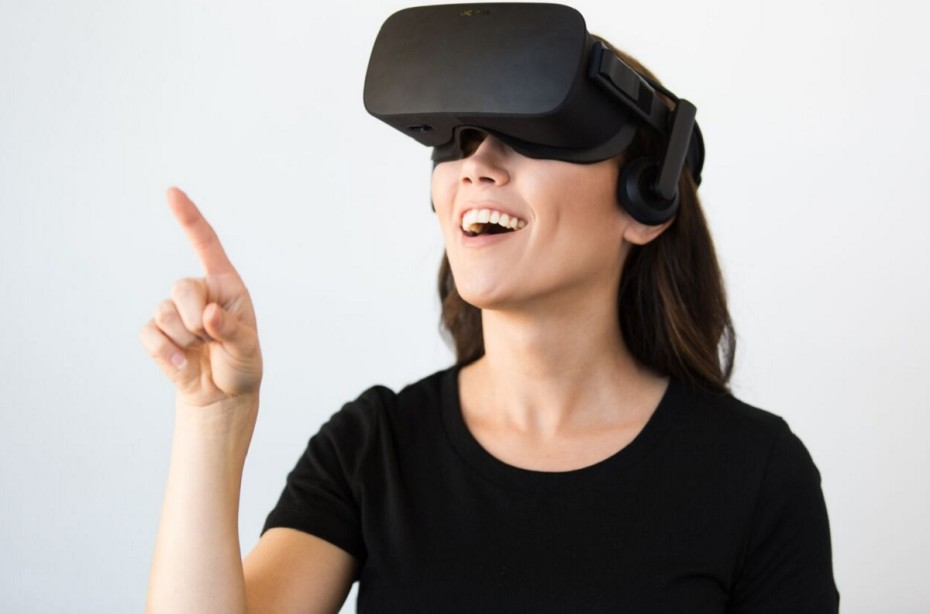
\includegraphics[width=\textwidth]{VR}
    %\vspace{-0.3cm}
\end{figure}
\noindent Ultimamente si parla sempre più spesso di \textit{Realtà Virtuale} ma cos'è, come si crea e a cosa serve?
Il termine \textit{Realtà Virtuale} fu coniato nel 1989 da Jaron Lanier, una delle prime persone che iniziò a lavorarci. Con il termine Realtà virtuale (Virtual Reality) si indica una Realtà simulata che si realizza attraverso la ricostruzione di ambienti o oggetti in modo da dare al soggetto una percezione il più possibile realistica della loro esistenza. A questa definizione tecnica si può a affiancare una più generale, che vede la Realtà virtuale come una Realtà parallela. è possibile distinguere due tipi di Realtà virtuale: una immersiva e una non immersiva. Si definisce immersiva la Realtà virtuale che è in grado di assorbire l'utente, realizzando una vera e propria immersione dei sensi nell'ambiente tridimensionale generato dal computer. Ciò è possibile attraverso l'utilizzo di dispositivi particolari: un visore, che permette la visualizzazione delle immagini tridimensionali e l'isolamento dall'ambiente esterno, ed un tracker, per il rilevamento di posizione e movimento dell'utente. Oltre a questi ne esistono molti altri, di cui alcuni ancora in fase di studio e perfezionamento. La Realtà virtuale non immersiva, invece, è caratterizzata dall'utilizzo di un monitor per la visualizzazione delle immagini tridimensionali e non si serve dell'ausilio di un tracker determinando nell'utente la sensazione di vedere il mondo tridimensionale, creato dal computer, come attraverso "una finestra" e in maniera quindi non partecipativa.
\section{Come si crea la Realtà Virtuale}
La Realtà Virtuale è possibile grazie a strumenti, programmi e linguaggi di programmazione appositi. Nella tesi proposta, si è scelto di utilizzare una Realtà Virtuale di tipo immersivo. Questa tipologia richiede una strumentazione più complessa e performante rispetto alla tipologia non immersiva. Gli strumenti che richiede, sono i seguenti:
\begin{itemize}
  \item \textbf{Computer}: tutte le periferiche utilizzate fanno capo a un hardware, se non integrato, che funge da fulcro per l’elaborazione e lo smistamento dei dati. Questo fulcro è spesso rappresentato da un computer dalle prestazioni elevate, in termini di CPU e GPU. La sua funzione, oltre a mantenere uno stato aggiornato, è quella di ricevere dati da sensori esterni, utili per recepire le azioni dell’utilizzatore, e inviare informazioni di feedback delle azioni elaborate. Ad esempio l’aggiornamento delle immagini visualizzate e l’attivazione di attuatori per altri tipi di sensazioni (ad esempi tattili).
	\item\textbf{Visore}: costituito da due pannelli LCD impostati per la vista bioculare, questo isola dal mondo esterno e costituisce una specie di casco. Questa impostazione dà la sensazione di tridimensionalità. Il visore può essere dotato di sensori in grado di rilevare i movimenti dell’utente come la rotazione del capo per inquadrare un’altra area del mondo virtuale. In alternativa, esistono visori economici che non sono altro che contenitori, muniti di lenti, che permettono di inserire lo smartphone e utilizzarlo come schermo LCD e come fulcro di tutte le funzioni hardware e software.
  \item \textbf{Auricolari}: solitamente integrati nei visori, permettono di udire i suoni emessi dal mondo virtuale. Il software deve variare i suoni emessi in base alla posizione dell'utilizzatore.
  \item \textbf{Sensori}: per il riconoscimento dei movimenti e delle azioni dell'utilizzatore. I sensori presenti nel visore danno informazioni sulla posizione, sul movimento della testa e del corpo. I sensori sono di vario tipo e sono in continuo sviluppo. I più conosciuti sono: guanti, in sostituzione dei canonici gestori di input (joystick, mouse, tastiere, ecc.); tute, in grado di trasferire le posture e i movimenti dell’utente nella rappresentazione e Virtuix Omni, una piattaforma che permette di muoversi camminando nell’ambiente virtuale.
\end{itemize}






















%
\chapter{Architettura del sistema Hardware}
\label{hardware}
\thispagestyle{empty}

\noindent In questo capitolo e nel successivo si descriverà la progettazione del sistema creato. Inizialmente si tratterà l'analisi del progetto e le scelte effettuate per quanto riguarda gli strumenti da utilizzare. Successivamente si descriveranno tutti i moduli che compongono l'architettura del sistema. La trattazione è divisa in parte hardware e parte software.

\noindent L'obiettivo del progetto è quello di creare uno strumento che permetta all'utilizzatore di pedalare, sterzare e osservare un luogo in un mondo virtuale. In primo luogo, era necessario creare un sistema simile ad una bicicletta. Ai fini di sperimentazione della tipologia di progetto, si è scelto di utilizzare una cyclette. La suddetta, permette di semplificare notevolmente il sistema elettronico e il sistema software, poiché questi non devono tenere conto dell'attrito e del ritorno di forza, in quanto una pedalata farà sempre ruotare il volano. La cyclette è inoltre sprovvista di freni, i quali potrebbero essere utilizzati per frenare la bicicletta virtuale. Si è quindi scelto di ottenere solo le informazioni relative alla pedalata e alla posizione del manubrio. Queste informazioni devono essere elaborate da un microcontrollore che ottiene i dati da tutti i sensori e genera una macro-informazione da inviare al sistema software.

\section{Sensori del manubrio}
\begin{figure}%
    \centering
    \subfloat[I 4 fotodiodi]{{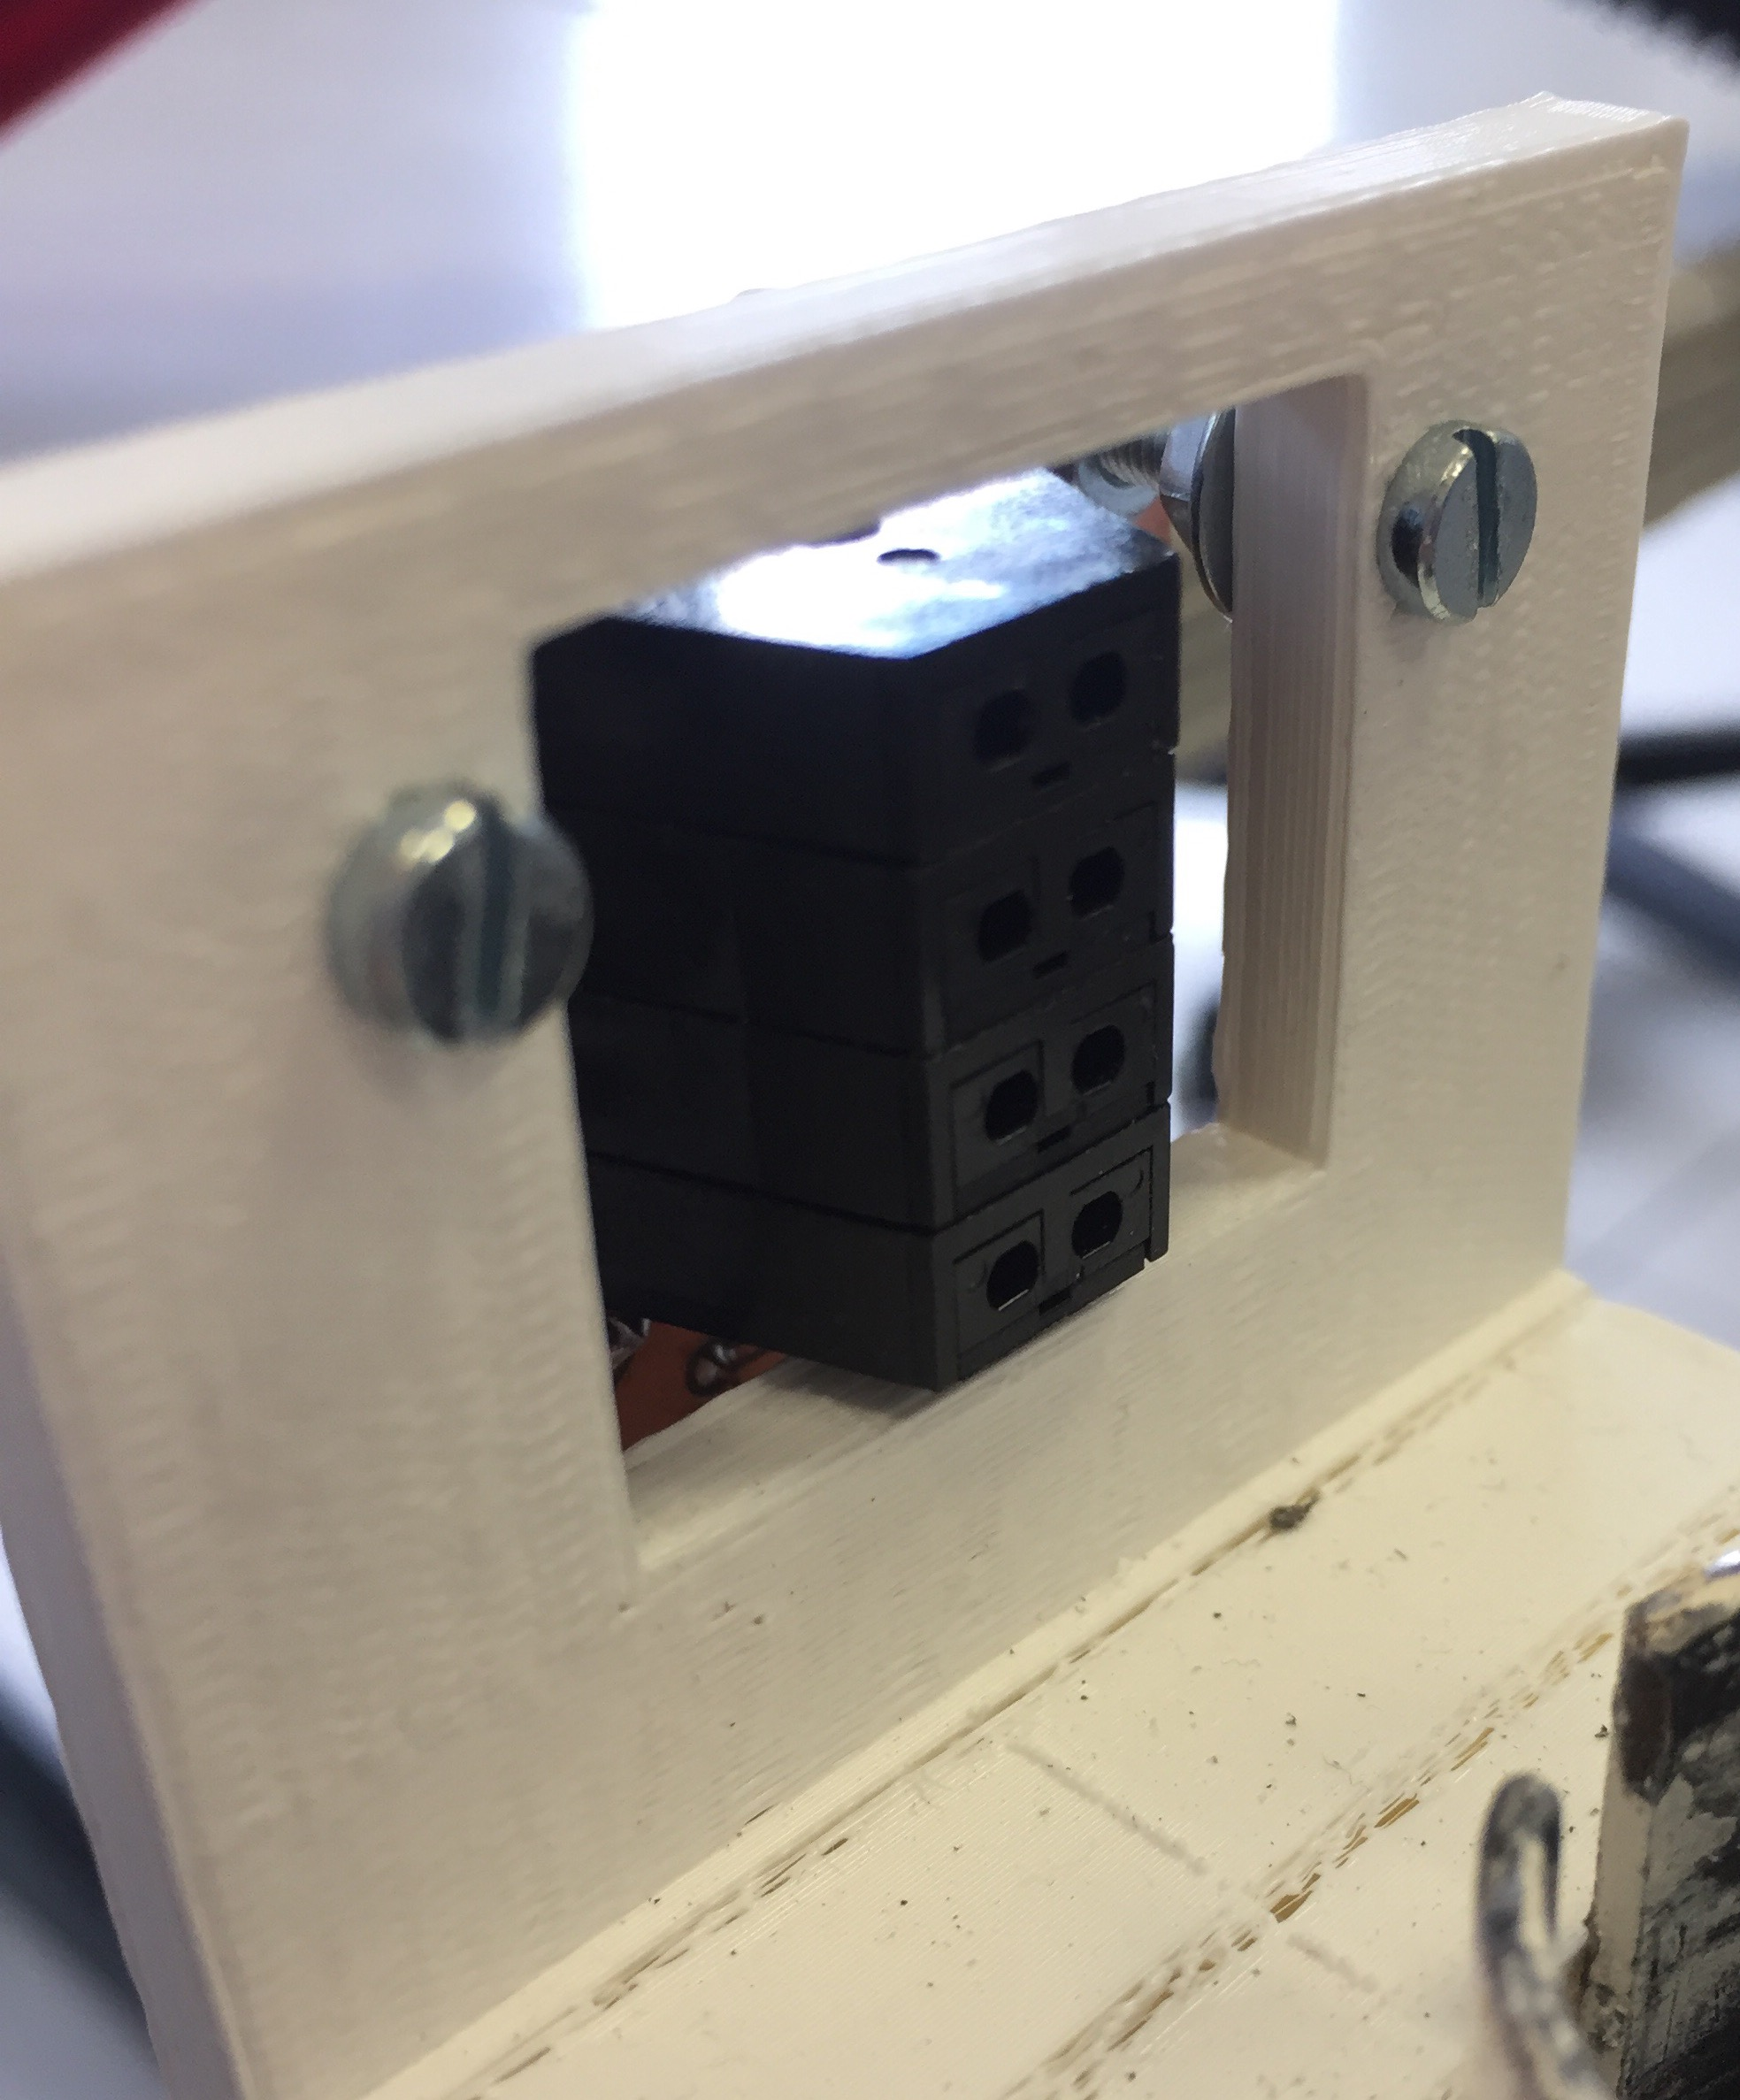
\includegraphics[height=5.5cm]{4Fotodiodi} }}%
    \subfloat[Le 16 posizioni in permutazione ciclica]{{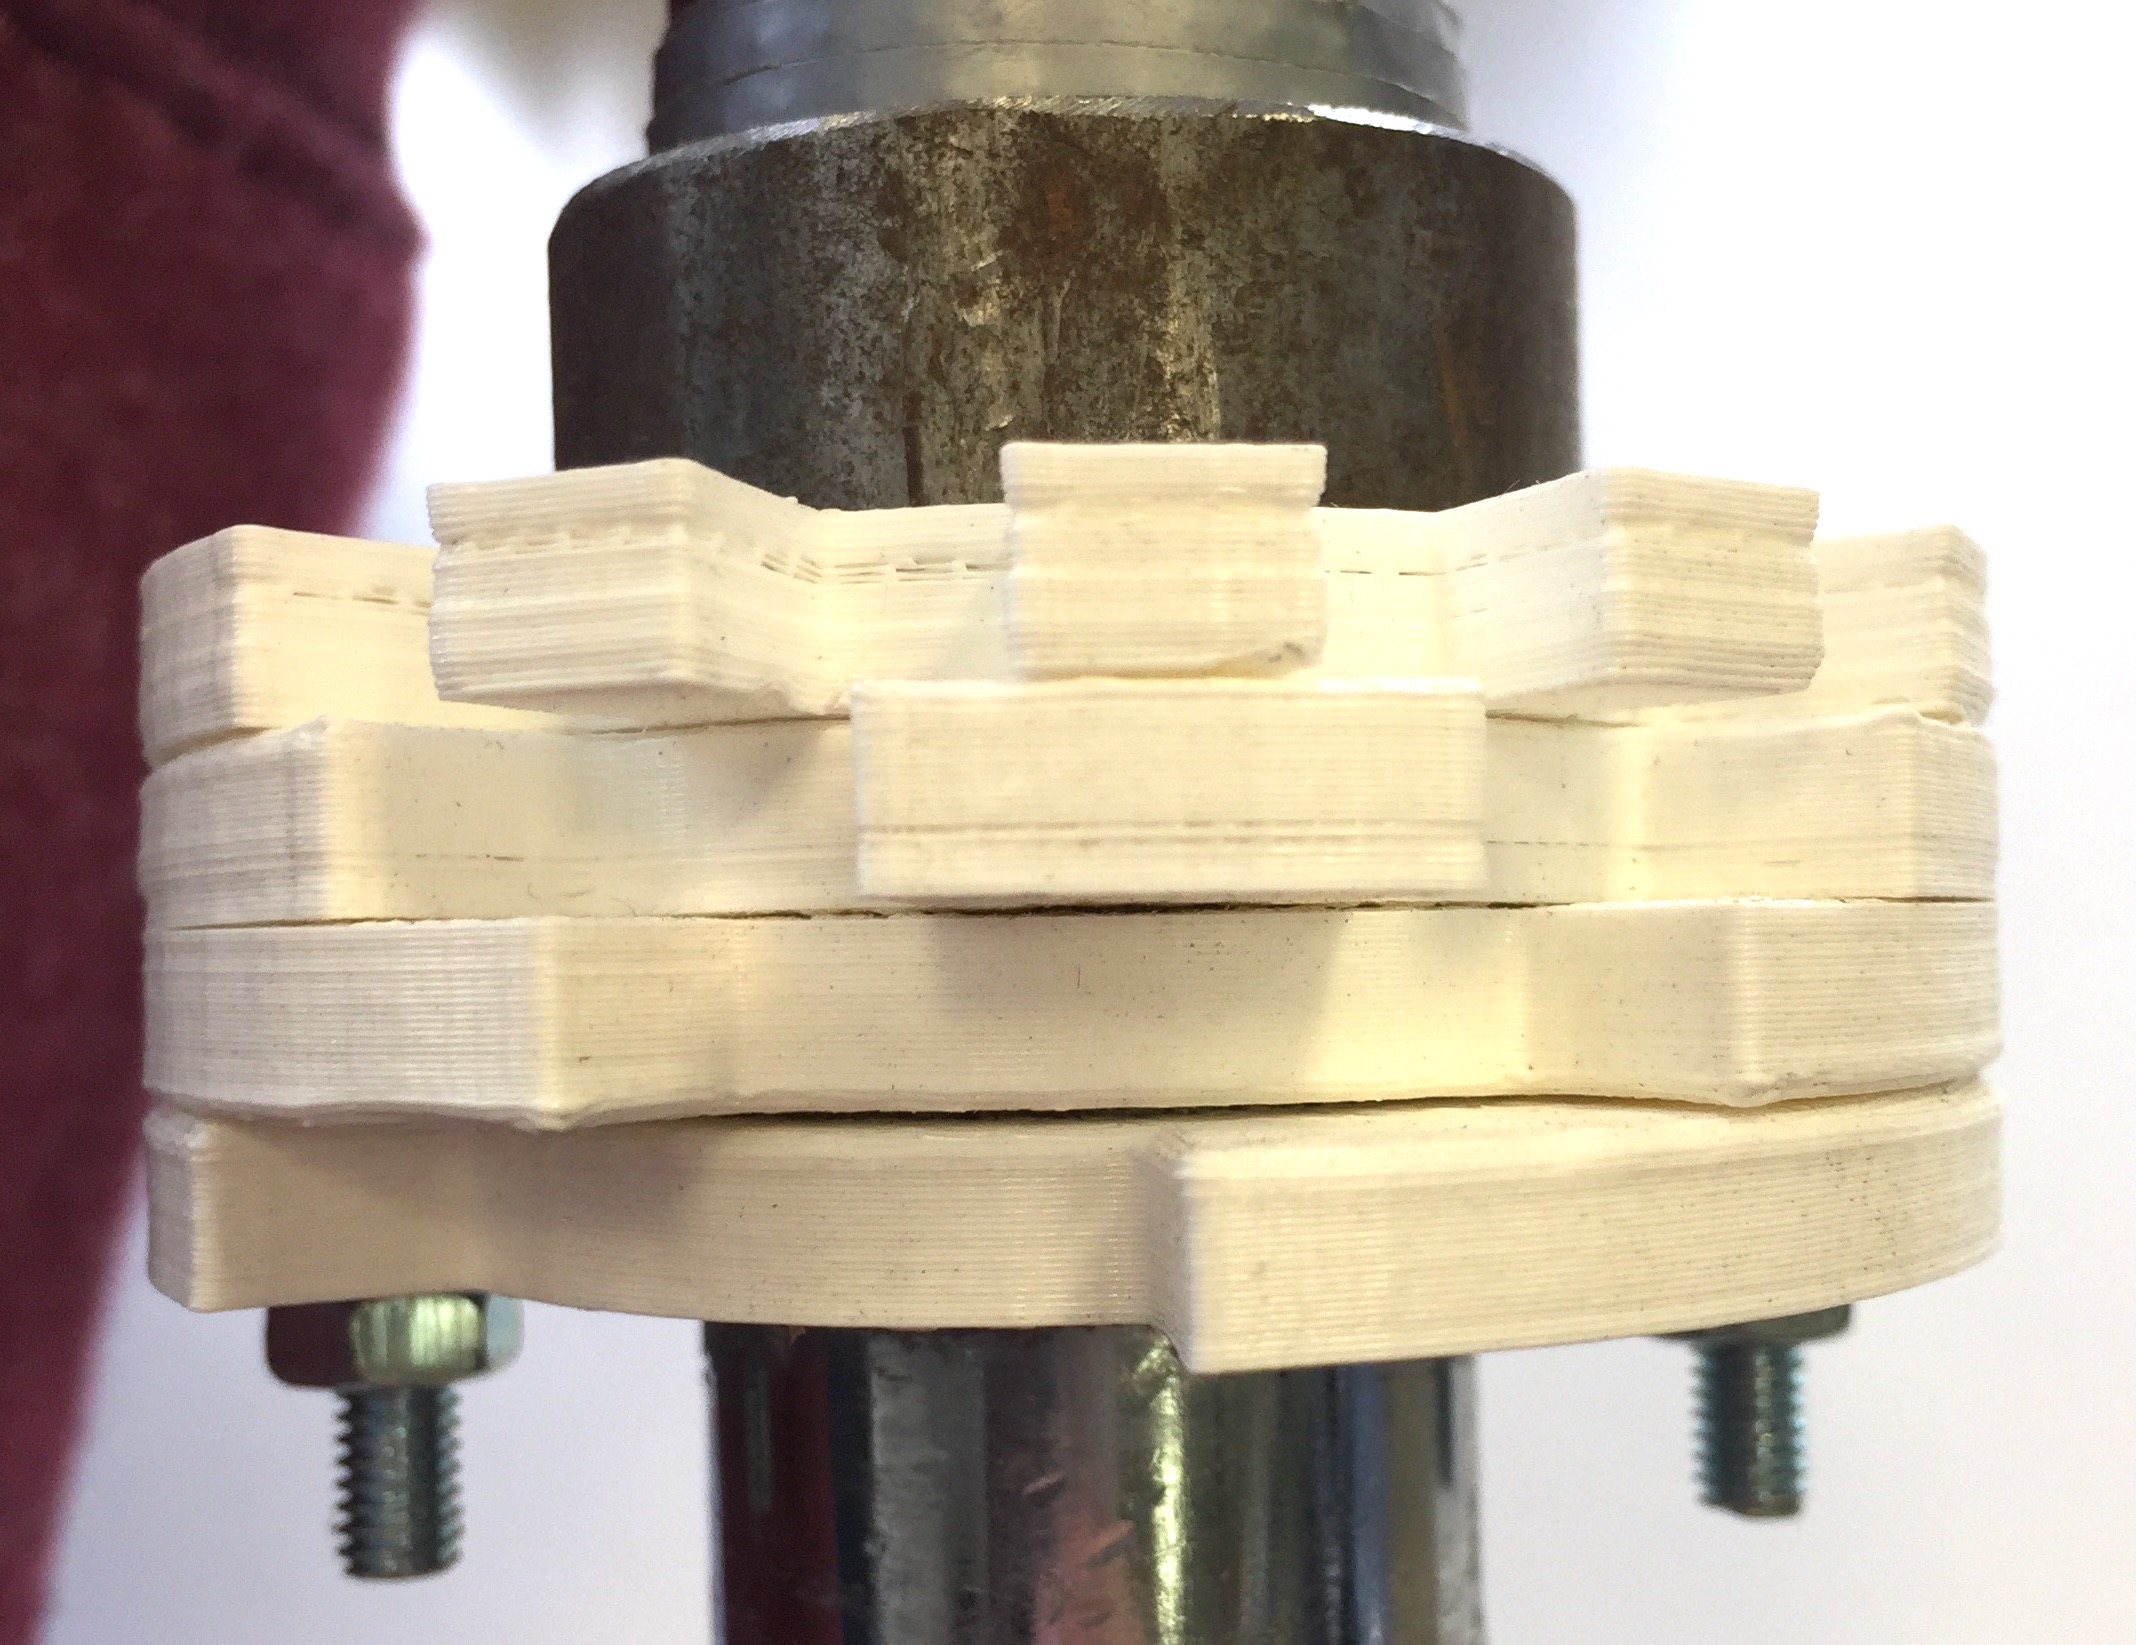
\includegraphics[height=5.5cm]{codifica4bitManubrio} }}%
    \caption{Sensori del manubrio}%
    \label{manubrio}
\end{figure}
Per ottenere le informazioni relative alla posizione del manubrio è stato scelto un angolo massimo di rotazione di 120\degree. Questo angolo è stato diviso in 16 posizioni. \\
\begin{wrapfigure}{r}{0.2\textwidth} %this figure will be at the right
    \centering
    \vspace{-1.5cm}
    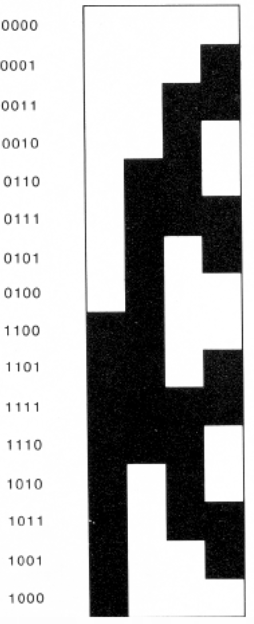
\includegraphics[width=0.2\textwidth]{codifica4bit}
\end{wrapfigure}
Per poter rilevare la posizione corrente è stata necessaria una codifica in 4 bit. Per ottenere questa codifica, si è fatto uso di 4 fotodiodi\footnote{Il fotodiodo è un particolare tipo di diodo fotorilevatore che funziona come sensore ottico sfruttando l'effetto fotovoltaico, in grado cioè di riconoscere una determinata lunghezza d'onda dell'onda elettromagnetica incidente e di trasformare questo evento in un segnale elettrico di corrente applicando ai suoi estremi un opportuno potenziale elettrico. Esso è dunque un trasduttore da un segnale ottico ad un segnale elettrico.} che permettono di rilevare i 4 spazi che compongono una delle delle 16 configurazioni. I fotodiodi permettono di distinguere uno spazio vuoto da uno spazio pieno creando un segnale elettrico. Le configurazioni sono state realizzate con un oggetto stampato con stampante 3D, come si vede in figura \ref{manubrio}b, in permutazione ciclica (figura a lato), che permette di accorpare gli \textit{uni} e gli \textit{zeri} e ridurre l'alternanza di \textit{vuoti} e \textit{pieni}.


\section{Sensori del volano}
\begin{figure}%

    \centering
    \subfloat[Fotodiodi]{{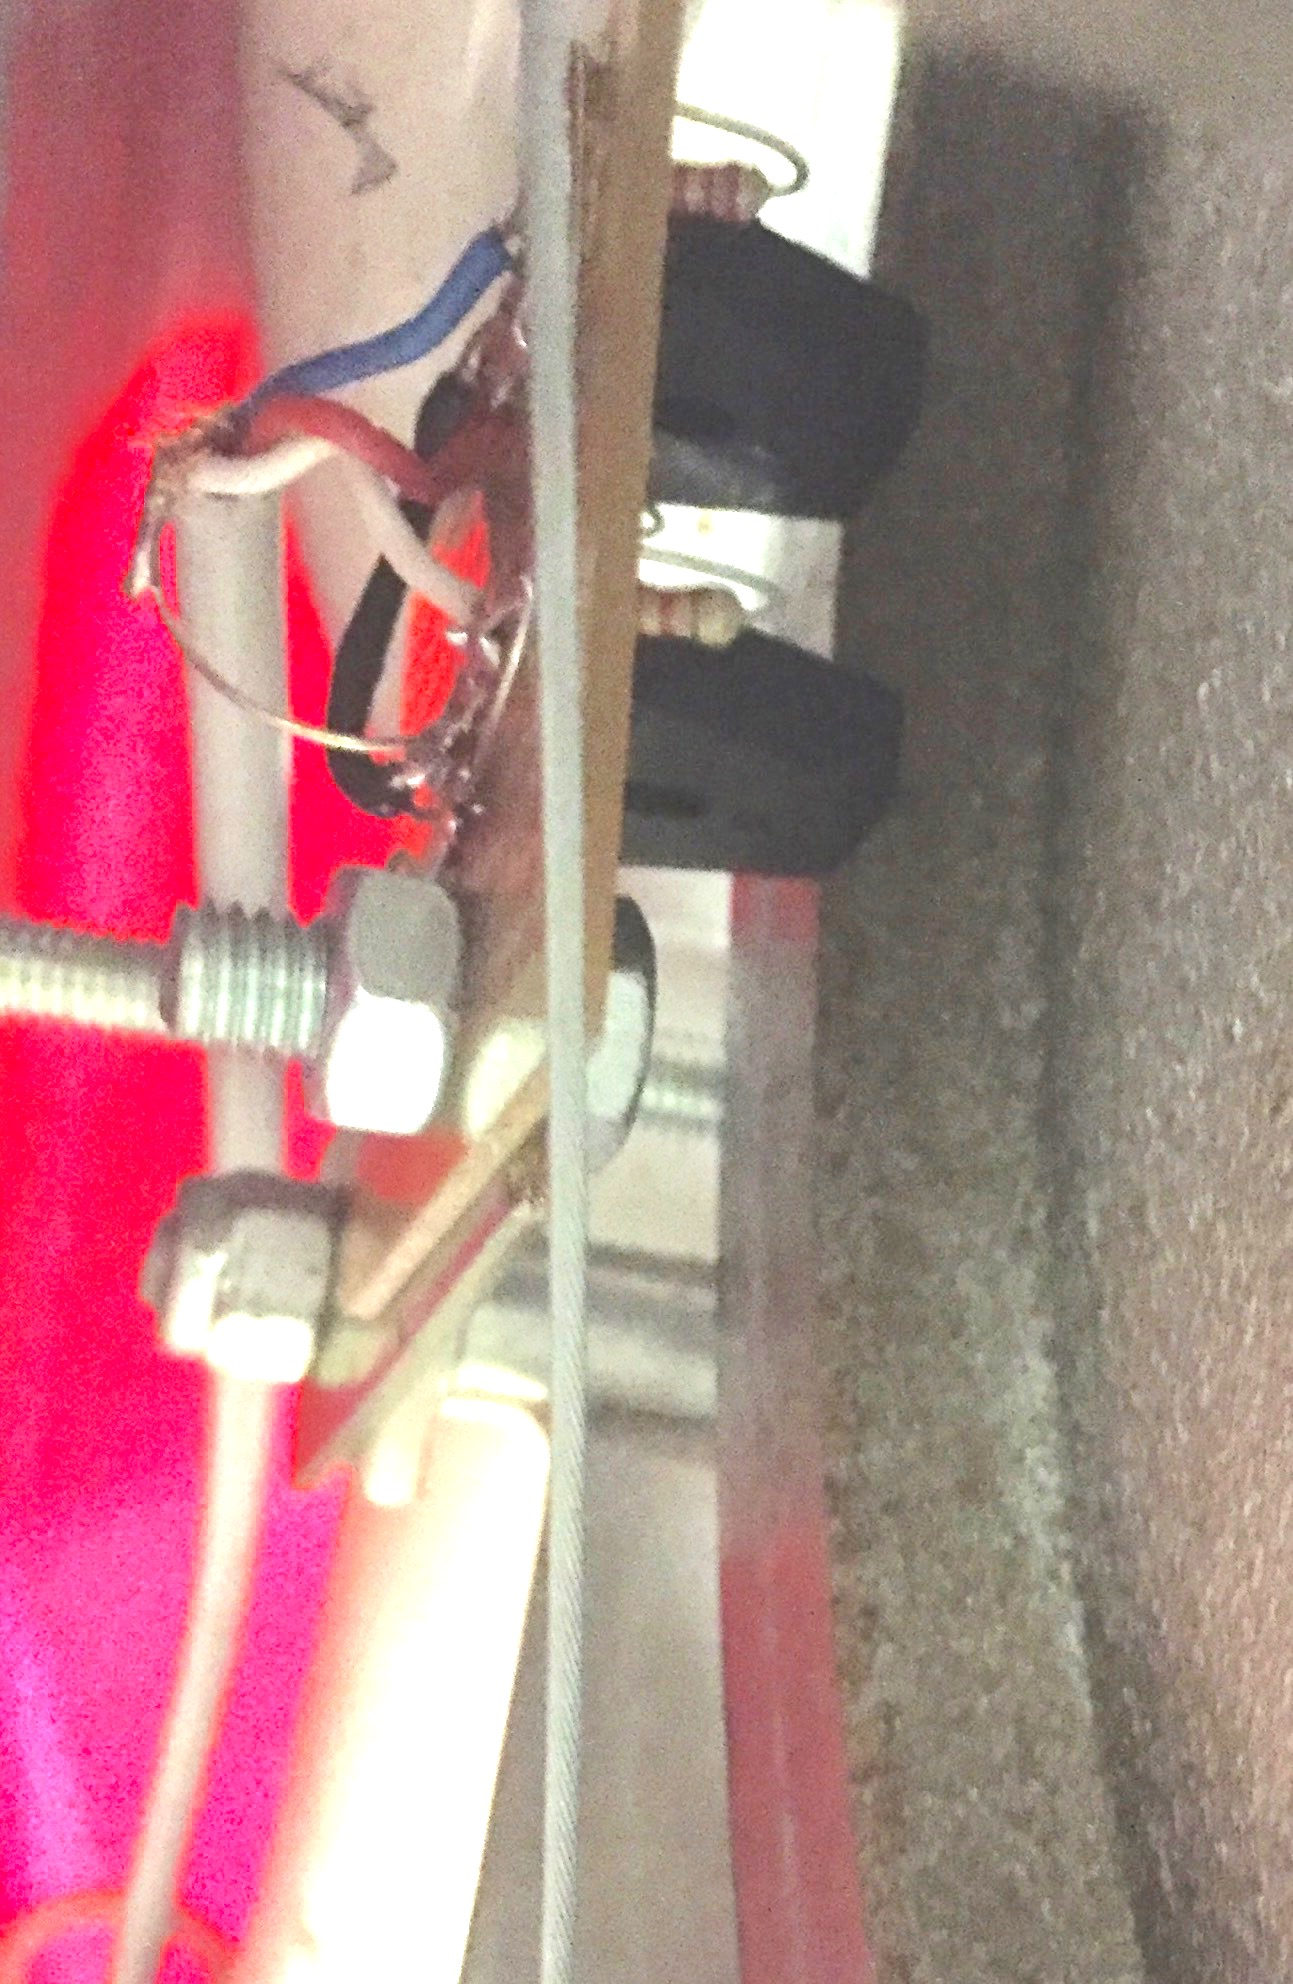
\includegraphics[height=6cm]{fotodiodivolano} }}%
    \subfloat[Polistirolo]{{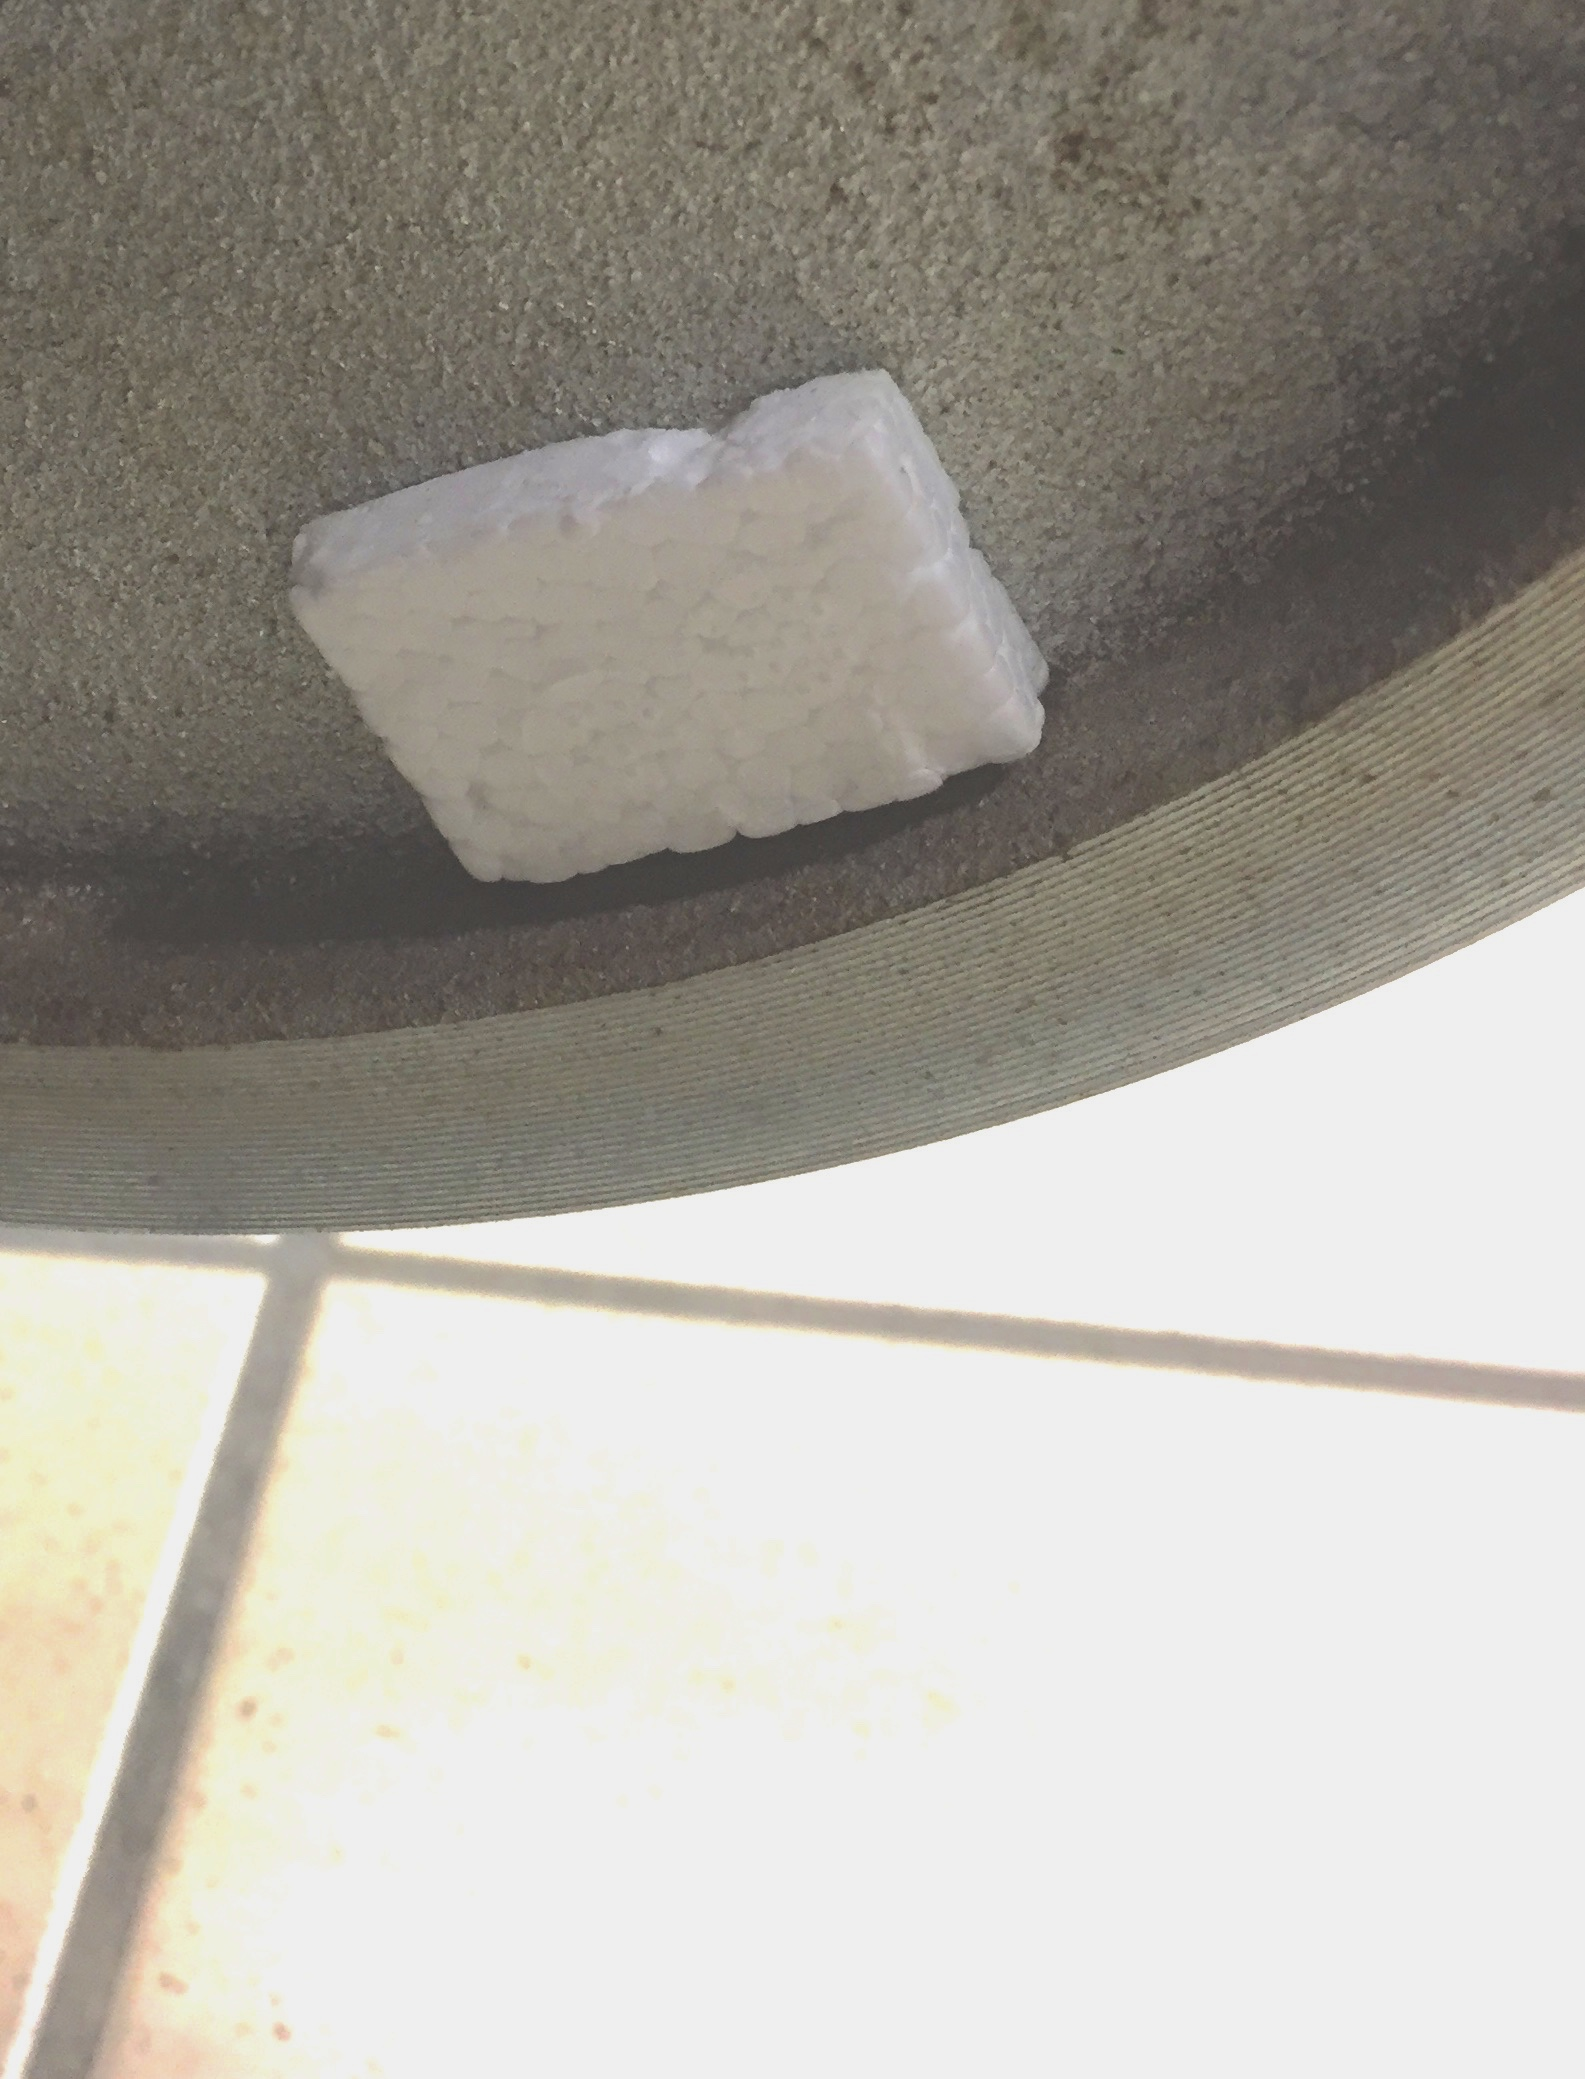
\includegraphics[height=6cm]{polistirolo} }}%
    \subfloat[Volano]{{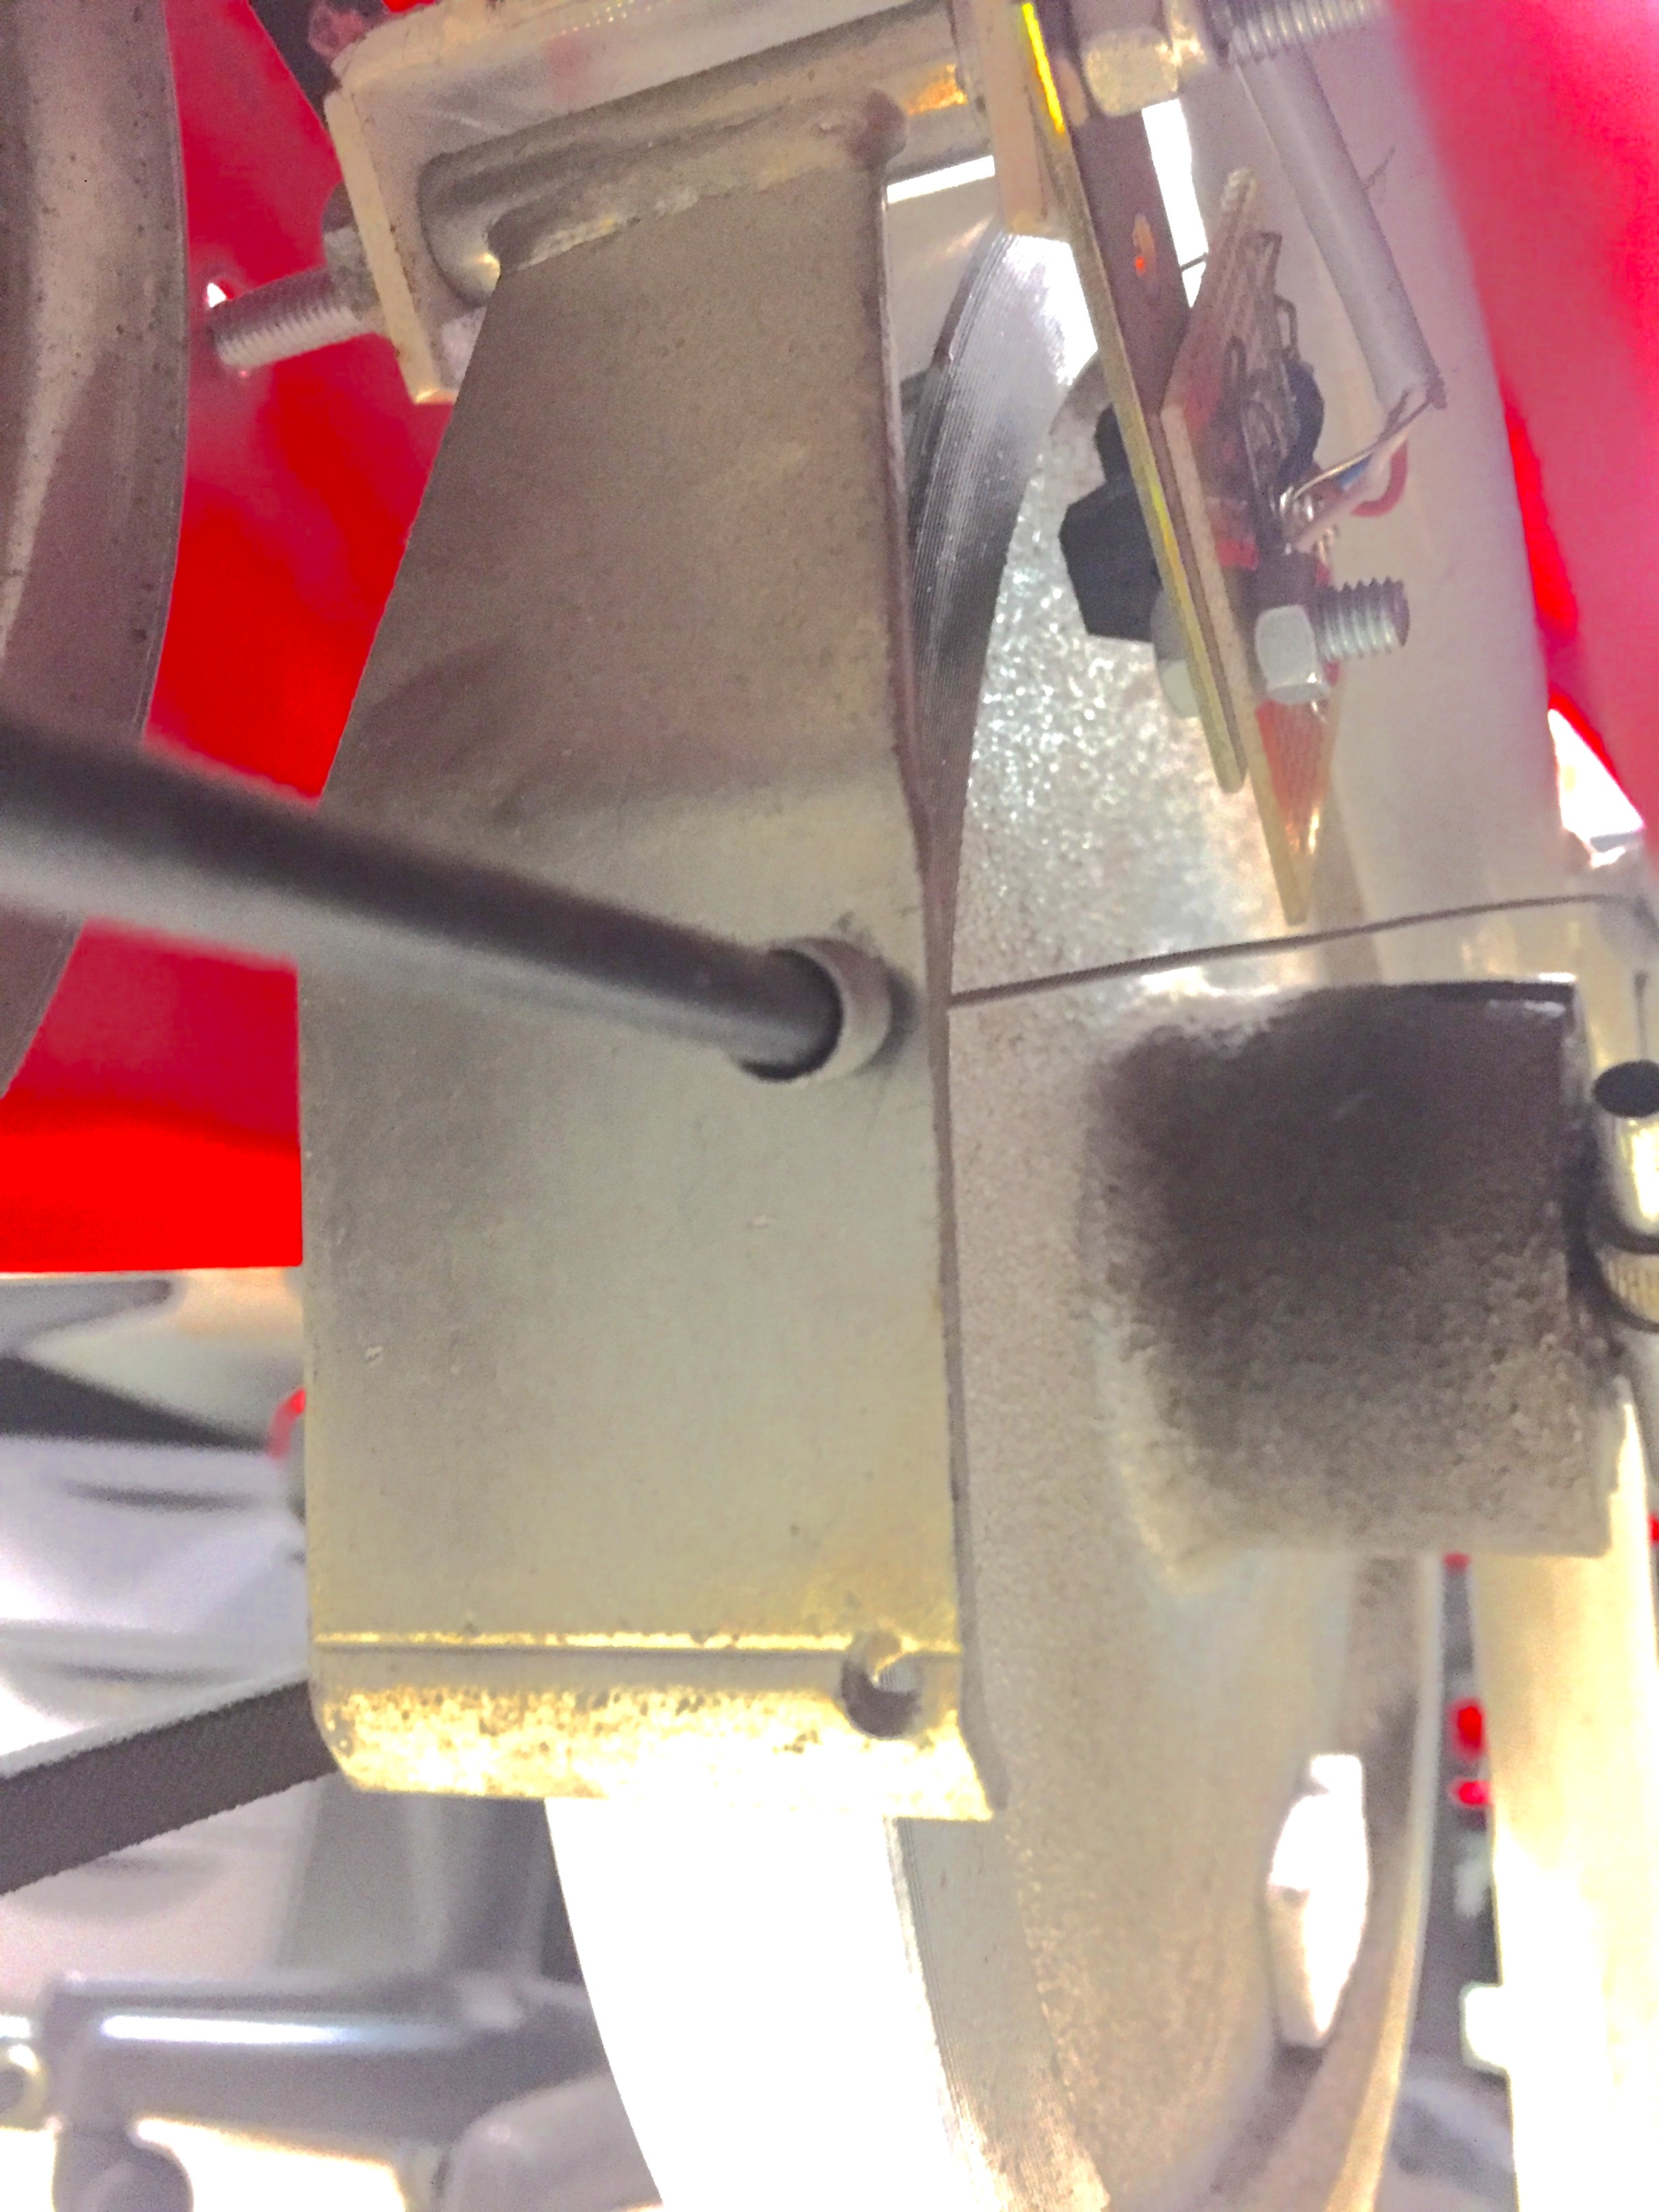
\includegraphics[height=6cm]{volano} }}%
    \caption{Sensori del volano}%
    \label{volano}
\end{figure}
La bicicletta virtuale deve muoversi ad una velocità consona alla rotazione del volano della cyclette. Quest'ultimo è stato quindi munito di un sistema che fornisce informazioni sulla velocità di rotazione. Il sistema di sensori è composto da due fotodiodi (figura \ref{volano}a) che permettono di ottenere la velocità di rotazione e distinguere se questa è oraria o antioraria. A questo fine, è stato installato sul volano un pezzo di polistirolo(figura \ref{volano}b) che permette di attivare i fotodiodi al passaggio. Grazie a questo, il microcontrollore può ottenere il tempo impiegato dal volano per coprire lo spazio che intercorre tra un fotodiodo e l'altro. La velocità di rotazione è quindi ottenuta tramite formula fisica della velocità, ovvero spazio percorso fratto tempo impiegato. La direzione di rotazione viene ottenuta distinguendo quale dei due fotodiodi viene attivato per primo. Ad esempio, se consideriamo due fotodiodi disposti orizzontalmente:\\
\begin{itemize}
  \item Se un oggetto passa da sinistra a destra, si oscurerà prima il fotodiodo sinistro poi il destro, quindi assumendo un oggetto che abbia il fulcro di rotazione sotto i fotodiodi, la sua rotazione è \textbf{oraria}
  \item in caso contrario, la rotazione è \textbf{antioraria}.
\end{itemize}
In figura \ref{volano}c si può osservare l'intero sistema del volano.

\section{Microcontrollore}
\begin{wrapfigure}{r}{0.4\textwidth} %this figure will be at the right
    \centering
    \vspace{-1.3cm}
    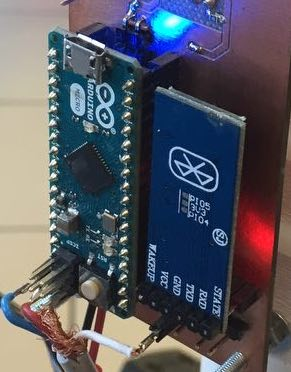
\includegraphics[height=5.5cm]{arduino}
    \caption{La scheda Arduino Micro e il modulo bluetooth}
    \vspace{-1.3cm}
\end{wrapfigure}

%=========CHIEDI a lanzoni come viene ottenuto il dato dall'accelerometro e come viene ottenuto il + e il -
Il cuore della parte hardware è la scheda Arduino che elabora tutti i dati ricevuti via cavo o via bluetooth. La scheda con il microcontrollore è in continua comunicazione in input e in output con il modulo bluetooth poiché deve ricevere l'informazione sulla rotazione dall'accelerometro e deve inviare all'elaboratore esterno una stringa contenente tutte le informazioni sotto forma di stringa.

\subsection{Stringa composta dal microcontrollore}
\label{stringa}
La stringa elaborata dall'Arduino è composta come segue:
\begin{itemize}
  \item \textbf{Posizione del manubrio}: un valore compreso tra 0 e 15 che indica la posizione del manubrio
  \item \textbf{Velocità di rotazione}: un valore compreso tra 0 e 40 che indica la velocità di rotazione della pedalata.
  \item \textbf{Senso di rotazione}: un segno \textbf{+} o \textbf{-} che indica senso orario o antiorario di rotazione della pedalata.
\end{itemize}

\noindent Un esempio pratico è \textbf{12+27.5}: significa che si sta registrando una pedalata in senso orario con velocità 27.5 e il manubrio è nella posizione 12.

\section{Ricevitore Bluetooth}
La ricezione della stringa avviene tramite un ricevitore bluetooth collegato ad una porta USB del computer generale in cui viene eseguito il software. Utilizzando un programma terminale apposito, chiamato HyperTerminal è stato possibile leggere la porta seriale COM a cui vengono inviati i dati a 9600 bit/s e testare la parte hardware.

\section{OSVR}
\begin{figure}[htb]
    \centering
    \vspace{-0.7cm}
    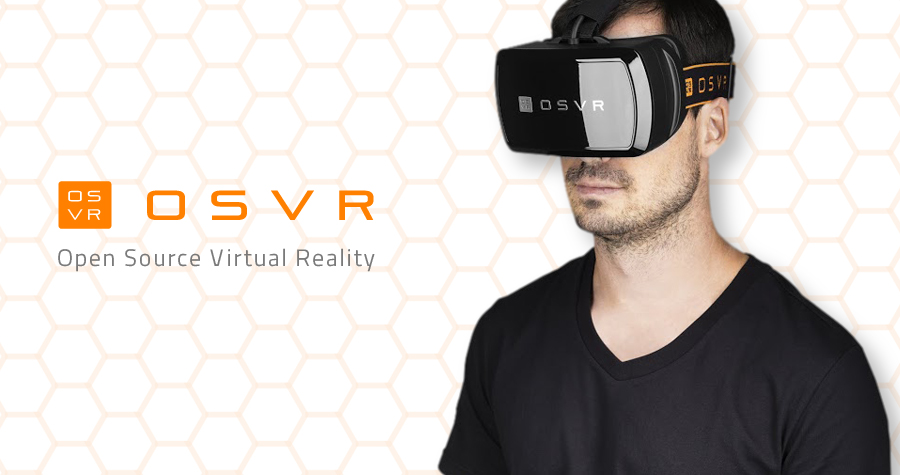
\includegraphics[width=\textwidth]{osvr1}
    \vspace{-1cm}
\end{figure}
\noindent OSVR é l'acronimo di \textit{Open-Source Virtual Reality} ed identifica la piattaforma software open-source per la Realtà Virtuale e quella aumentata. \\È stata sviluppata dalla Razer e da Sensics. La prima è l'azienda leader nel settore del gaming, mentre la seconda lo è nel settore della realtà virtuale. Affinché questa piattaforma sfondasse nel mercato, le società sopracitate hanno deciso di rendere open-source sia il software sia l'hardware per i programmatori. È infatti reperibile su github il codice sorgente. OSVR consente in modo davvero semplice la configurazione e la gestione dei vari dispositivi: occhiali VR, inseguitori di posizione, periferiche di gioco e vari altri. 

\subsection{Caratteristiche}
L'OSVR è composto da un display montato su una visiera, o meglio head-mounted (HMD), da 2 lenti amovibili, da un display OLED da 5.5 pollici con risoluzione 1920 x 1080 pixel, 60 fps di refresh rate e campo visivo di 100 gradi. Contiene una scheda madre riprogrammabile con accelerometro e giroscopio integrati. Il visore OSVR dispone di doppie lenti che consentono di ridurre la distorsione delle immagini. A differenza di altri visori, questo dispone di una cintura elastica che porta i cavi fino all'altezza del muscolo trapezio dell'utilizzatore, in modo da non limitarne il movimento e quindi l'esperienza di gioco.\newpage

 \begin{figure}[htb]
    \centering
    %\vspace{-0.7cm}
    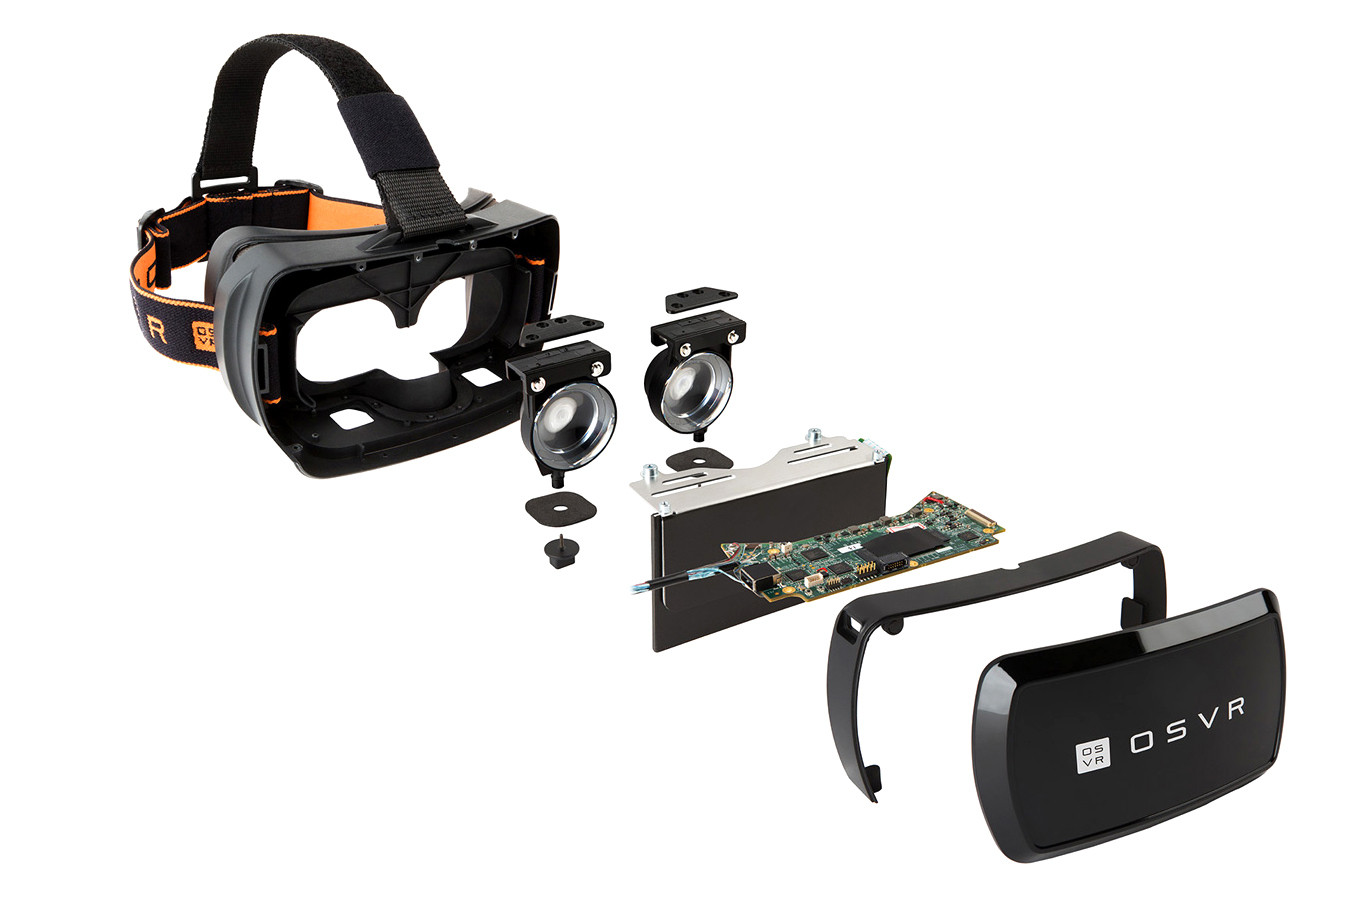
\includegraphics[height=8cm]{osvr2}
    \caption{I componenti del visore OSVR HDK1\label{fig:osvr2}}
    %\vspace{-0.3cm}
\end{figure}
\noindent Il punto forza di questa piattaforma è la facile integrazione con dispositivi e con software aggiuntivi. Ad esempio, utilizzando una telecamera eye-tracking è possibile adoperare il software fornito dal produttore della fotocamera per calcolare la direzione dello sguardo. È inoltre possibile utilizzare il visore in praticamente il 90\% dei sistemi operativi.
In questo modo lo sviluppatore non ha più bisogno di scegliere anticipatamente un particolare sistema operativo per la sua applicazione, la cui realizzazione richiederà meno tempo sfruttando i plug-in dei quali l'OSVR dispone. Si permette così allo sviluppatore di concentrarsi su essa piuttosto che sull'interfacciamento.
 Sono inoltre reperibili all'interno di Github\footnote{GitHub è un servizio di hosting per progetti software. Il nome deriva dal fatto che è un servizio sostitutivo del software dell'omonimo strumento di controllo versione distribuito, Git.}, tutti i plug-in di integrazione con i vari motori grafici quali Unity e Unreal Engine.
\subsection{Integrazione}
L'integrazione dell'OSVR verrà trattata nella sezione \textit{\nameref{software}} in cui si descriverà il procedimento per installare, configurare ed utilizzare il visore.
\chapter{Architettura del sistema Software}
\label{software}
\thispagestyle{empty}

%============PARTE SOFTWARE=============%
\label{software}
La parte software è stata scritta interamente nel linguaggio \Csharp\: e si avvale del motore grafico Unity. L'applicazione crea un'ambientazione virtuale in cui viene posizionata una bicicletta a cui viene collegato uno script che legge continuamente la porta COM su cui il microcontrollore invia la stringa contente l'informazione di movimento. Lo script parsifica la stringa e dà i valori in pasto al motore grafico che muove la bicicletta virtuale.
\section{Blender}
\begin{wrapfigure}{r}{0.2\textwidth} %this figure will be at the right
    \centering
    \vspace{-1.0cm}
    
\includegraphics[height=2cm]{blender}
\end{wrapfigure}
Blender è un software libero e multipiattaforma di modellazione, animazione, compositing e rendering di immagini tridimensionali. Inoltre dispone di funzionalità per mappature UV e simulazioni di rivestimenti adatte alla creazione di applicazioni e giochi 3D. All'interno di Blender tutte le funzioni e le interfacce possono essere richiamate con scorciatoie e per questo motivo quasi tutti i tasti sono collegati a numerosi comandi. La sua interfaccia si basa essenzialmente sulla finestra principale di lavoro, in cui è possibile visualizzare un modello 3D e modificarlo. 
\begin{figure}[hbt]
\centering
  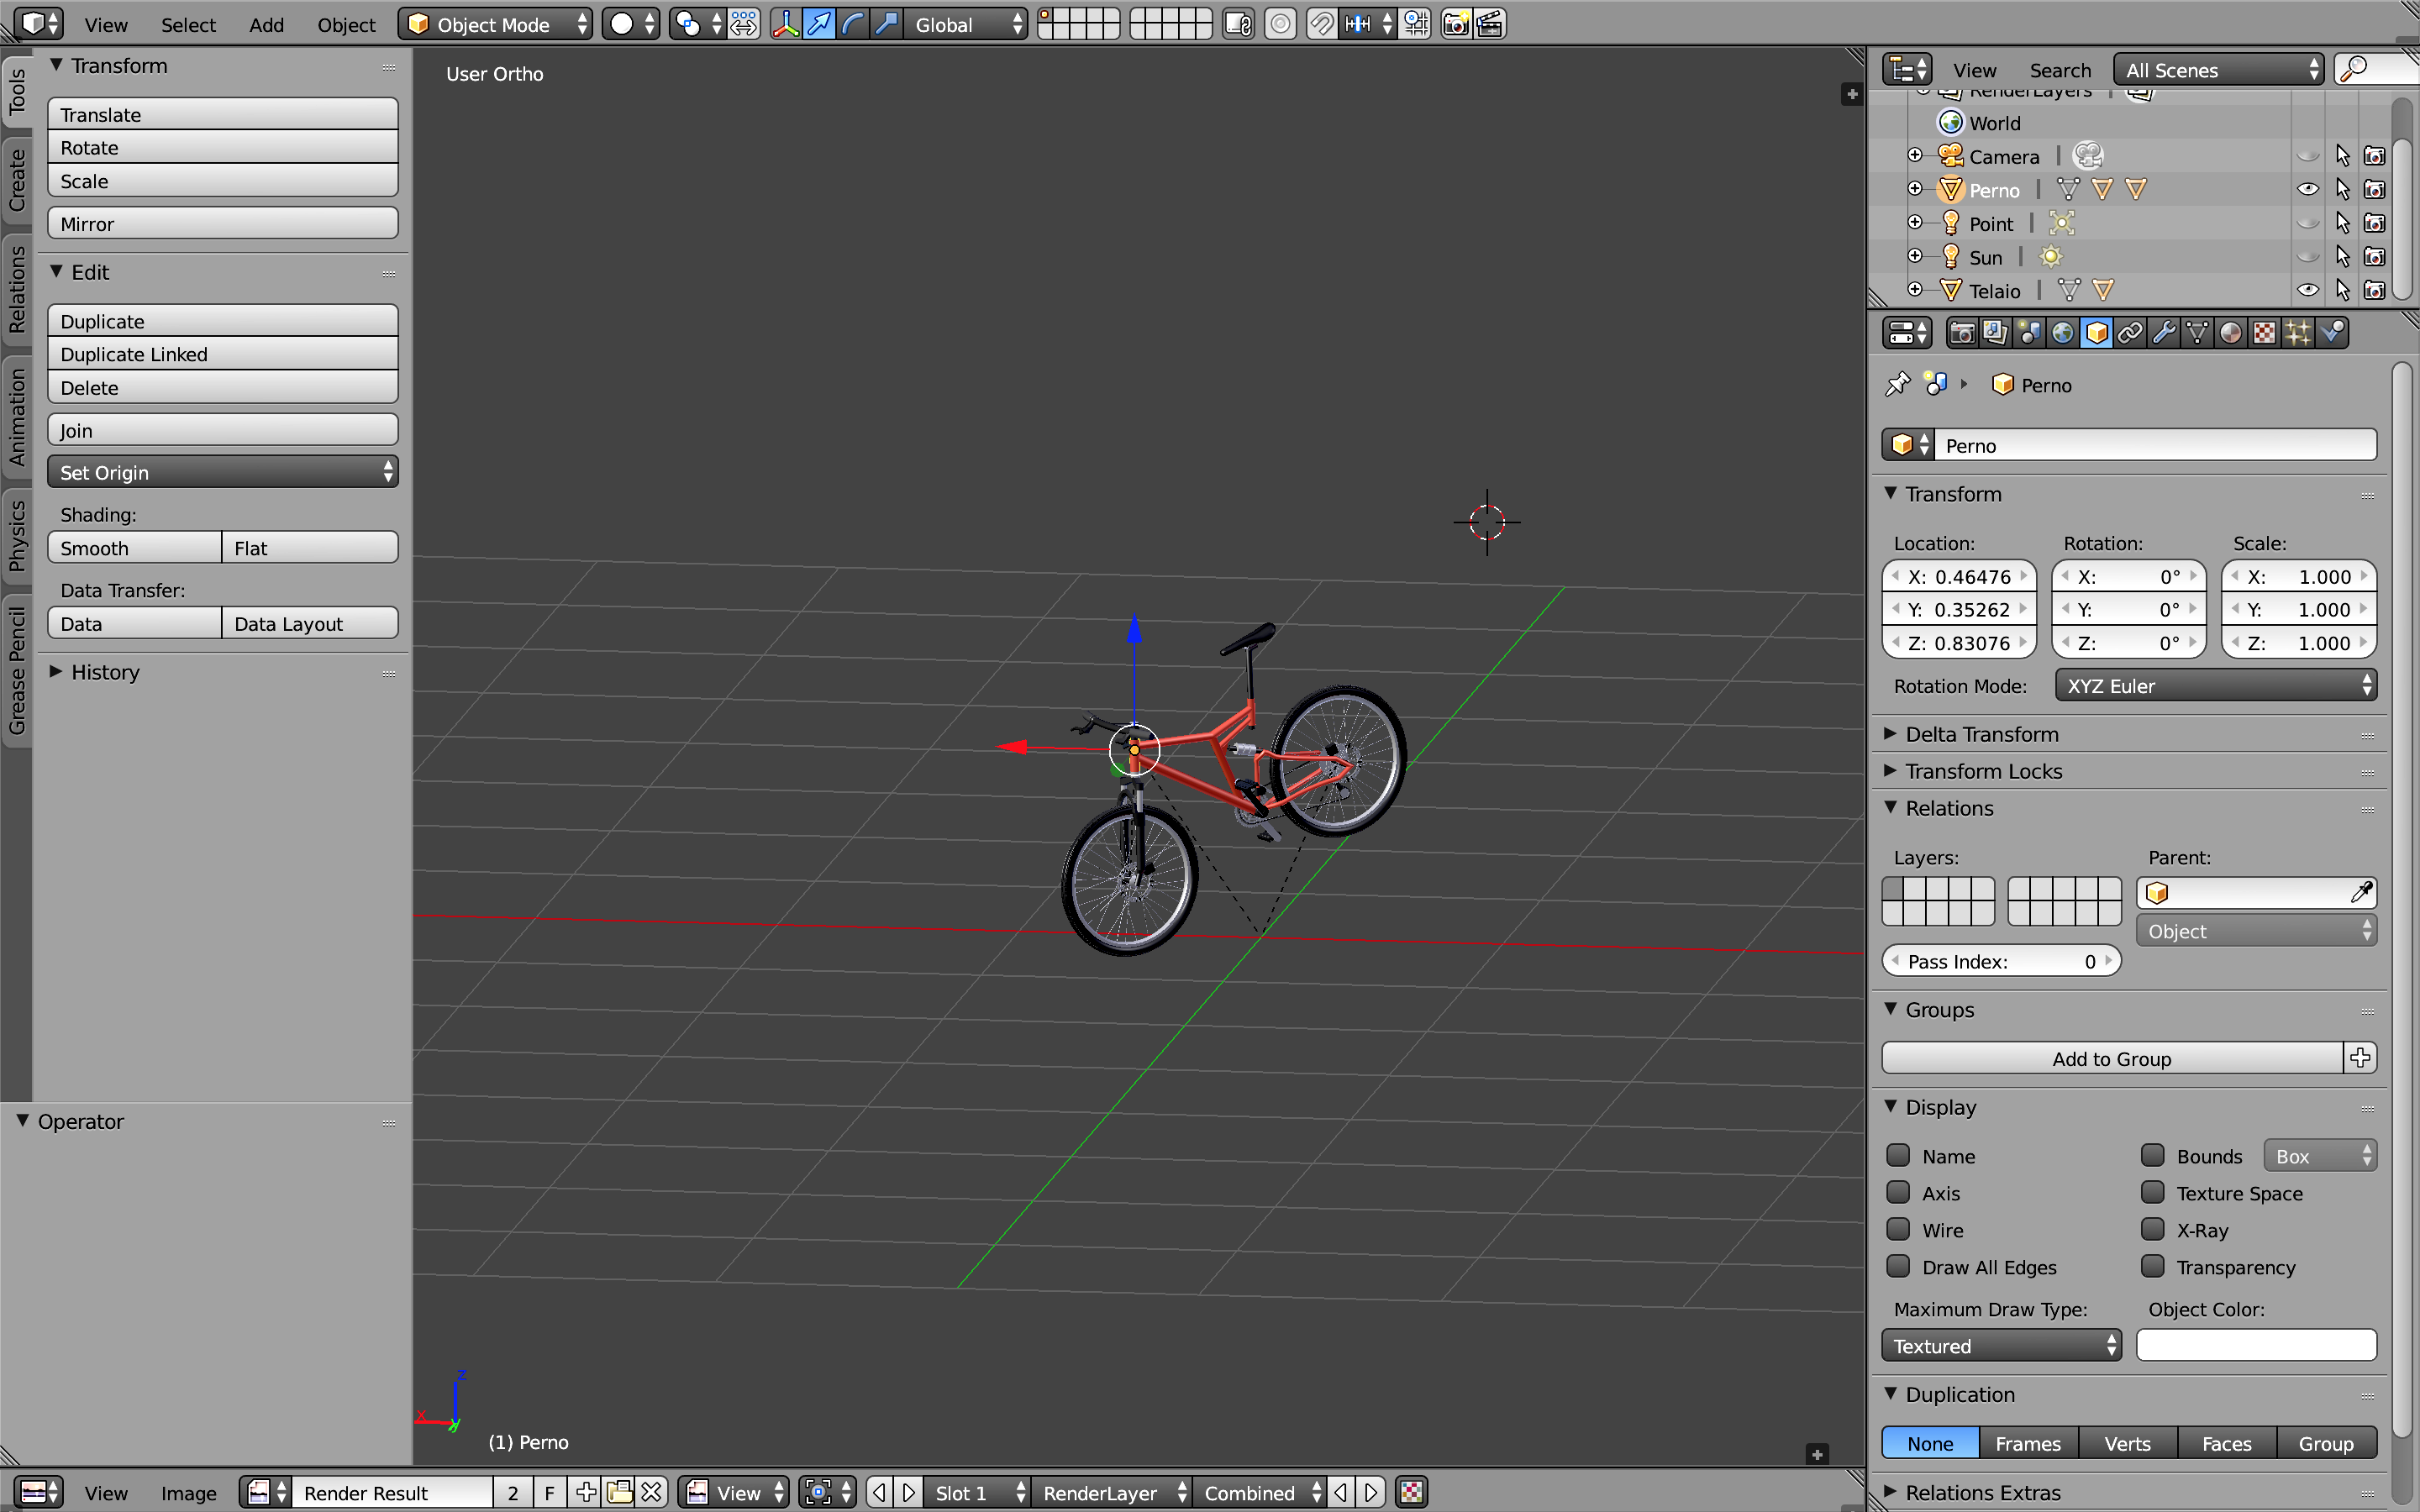
\includegraphics[height=8cm]{schermoblender.png}
  \caption{Interfaccia Principale di Blender}
\end{figure}

\noindent L'\textit{Object Mode} è la modalità che permette di visualizzare le mesh\footnote{Una mesh poligonale, anche detta maglia poligonale, è una collezione di vertici, spigoli e facce che definiscono la forma di un oggetto poliedrico nella computer grafica 3D e nella modellazione solida.} dell'oggetto, mentre l'\textit{Edit Mode} permette di modificarlo. Vi sono altre modalità che non sono state utilizzate, ma risultano utili per una modellazione più dettagliata. Per dotare il modello di texture o di materiali, ovvero l'applicazione di colori, trasparenza, lucentezza o altro, Blender implementa diverse finestre come la \textit{UV/Image Editor} nella quale è possibile scegliere la texture da applicare all'oggetto. Blender è stato utilizzato per creare la mesh della bicicletta virtuale da manovrare attraverso script collegati ad un motore grafico.
\subsection{Mesh della bicicletta}
%\begin{wrapfigure}{l}{0.5\textwidth} %this figure will be at the left
%    \centering
%    \vspace{-0.5cm}
%    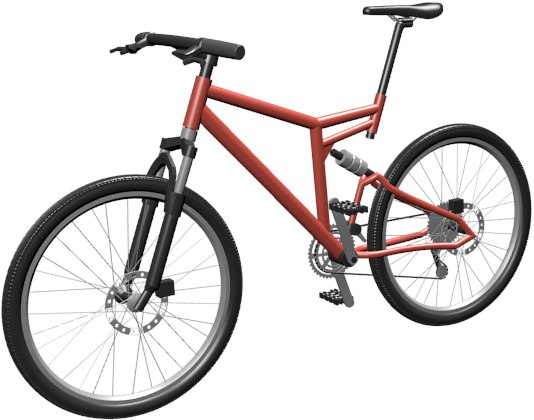
\includegraphics[height=5cm]{meshbici}
%\end{wrapfigure}
 \begin{figure}[htb]
    \centering
    %\vspace{-0.7cm}GameObject
    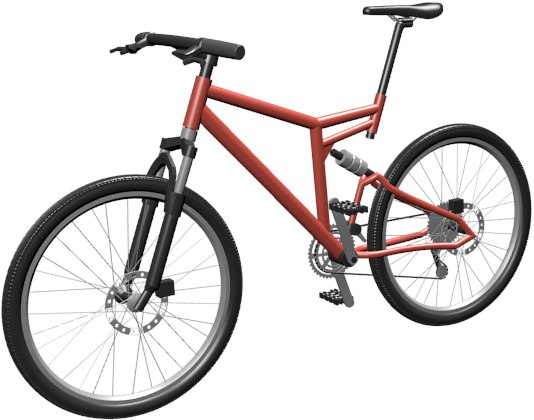
\includegraphics[height=8cm]{meshbici}
%    \caption{\label{fig:meshbici}}
    %\vspace{-0.3cm}
\end{figure}
\noindent La mesh proviene dal sito TurboSquid. È stata scaricata gratuitamente con estensione FBX\footnote{FBX è un formato di file di Autodesk che viene supportato dai più comuni software di grafica 3D in quanto è in grado di immagazzinare non solo geometrie, ma anche dati di texture e di animazioni.} ed è stata adattata per l'utilizzo necessario ai fini del progetto. È stata ridotta in scala ed è stata centrata alle coordinate (0,0,0). La mesh scaricata era già suddivisa in tutti i componenti di una bicicletta classica. Le uniche parti che devono essere dissociate ai fini della tesi sono il manubrio e il telaio. Sono state quindi assemblate tutte le mesh che compongono il telaio e tutte quelle che compongono il manubrio. Blender permette di associare un centro ad ogni mesh con la funzione \texttt{Set Origin > Origin to Geometry}. Questa permette di fornire, a tempo di esecuzione, una rotazione attorno al centro così definito. Sono state quindi lasciate libere le ruote e sono state centrate nel loro origine, in modo da poter dare una rotazione attorno al proprio asse.
\noindent La mesh della bicicletta è stata quindi suddivisa come segue:
\begin{itemize}
  \item \textbf{Telaio}: comprende tutto il telaio della bicicletta escluso il manubrio e le ruote.
	\begin{itemize}
  \item \textbf{Ruota posteriore}: è stata separata per darle possibilità di ruotare sul suo asse.
 \end{itemize}
  \item \textbf{Perno}: consiste nell'unione tra ruota e manubrio. Questo oggetto permette di ruotare tutto il manubrio mantenendo però un asse di rotazione inclinato. Comprende:
 \begin{itemize}
 \item \textbf{Manubrio}: contiene il manubrio stesso, la forcella e l'asse di sterzo.
 \item \textbf{Ruota anteriore}: è stata separata per darle la possibilità di ruotare sul suo asse.
 \end{itemize}
\end{itemize}

\begin{wrapfigure}{r}{0.35\textwidth} %this figure will be at the right
    \centering
    \vspace{-1.3cm}
    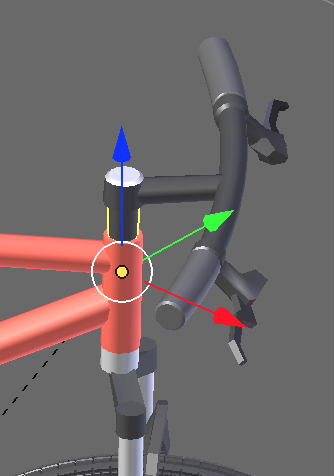
\includegraphics[height=5.5cm]{assebici}
    \caption{L'asse del canotto della bicicletta}
    \vspace{-1.3cm}
\end{wrapfigure}
\noindent Il telaio è stato separato dal manubrio solo nell'asse di sterzo, ma è stato mantenuto il canotto di sterzo, in modo da poter ruotare il manubrio attorno all'asse passante per il centro del canotto. La mesh così ottenuta è stata esportata ed è stata importata in Unity come oggetto da manovrare tramite script.\\
\subsection{Mesh dell'ambientazione}
\label{ambientazione}
\noindent Sono state utilizzate due diverse ambientazioni. La prima delle due è stata fornita dal Cineca: si tratta di un modello 3D dei portici di San Luca (Bologna) ottenuto tramite rilevazione laser. Il modello riporta fedelmente tutti i dettagli spaziali dei portici, ma non riportano la texture. La seconda ambientazione è stata scaricata gratuitamente dallo store di Unity. Per il progetto che è stato creato, l'ambientazione non ha alcuna rilevanza: è possibile asportare la bicicletta e posizionarla in un qualsiasi altro mondo virtuale, purché sia adatto al movimento di una bicicletta al suo interno. L'ambientazione può essere munita di luce principale sia su blender che sul motore grafico. L'importante è non sovrapporre troppe luci per non rischiare la sovra esposizione. In figura \ref{ambientazione} possiamo notare un esempio delle due ambientazioni.
\vspace{-0.5cm}
\begin{figure}[hbp]%
    \centering
    \subfloat[I portici di San Luca]{{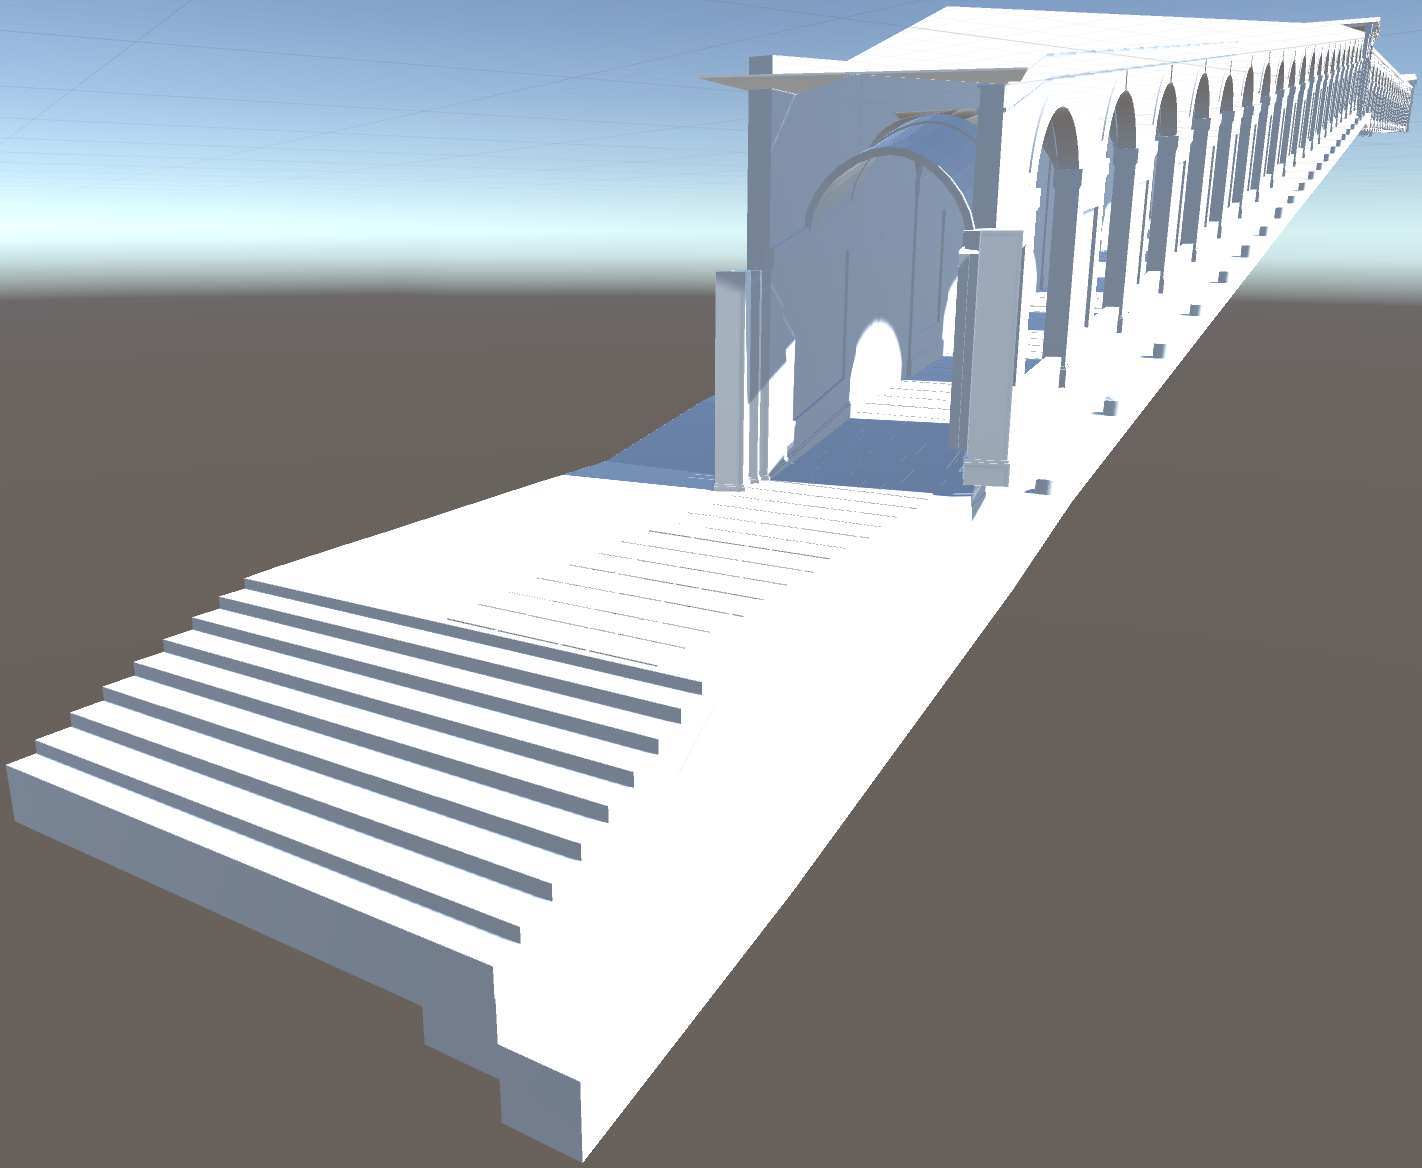
\includegraphics[height=5.5cm]{portici} }}%
    \subfloat[Il tracciato di gara]{{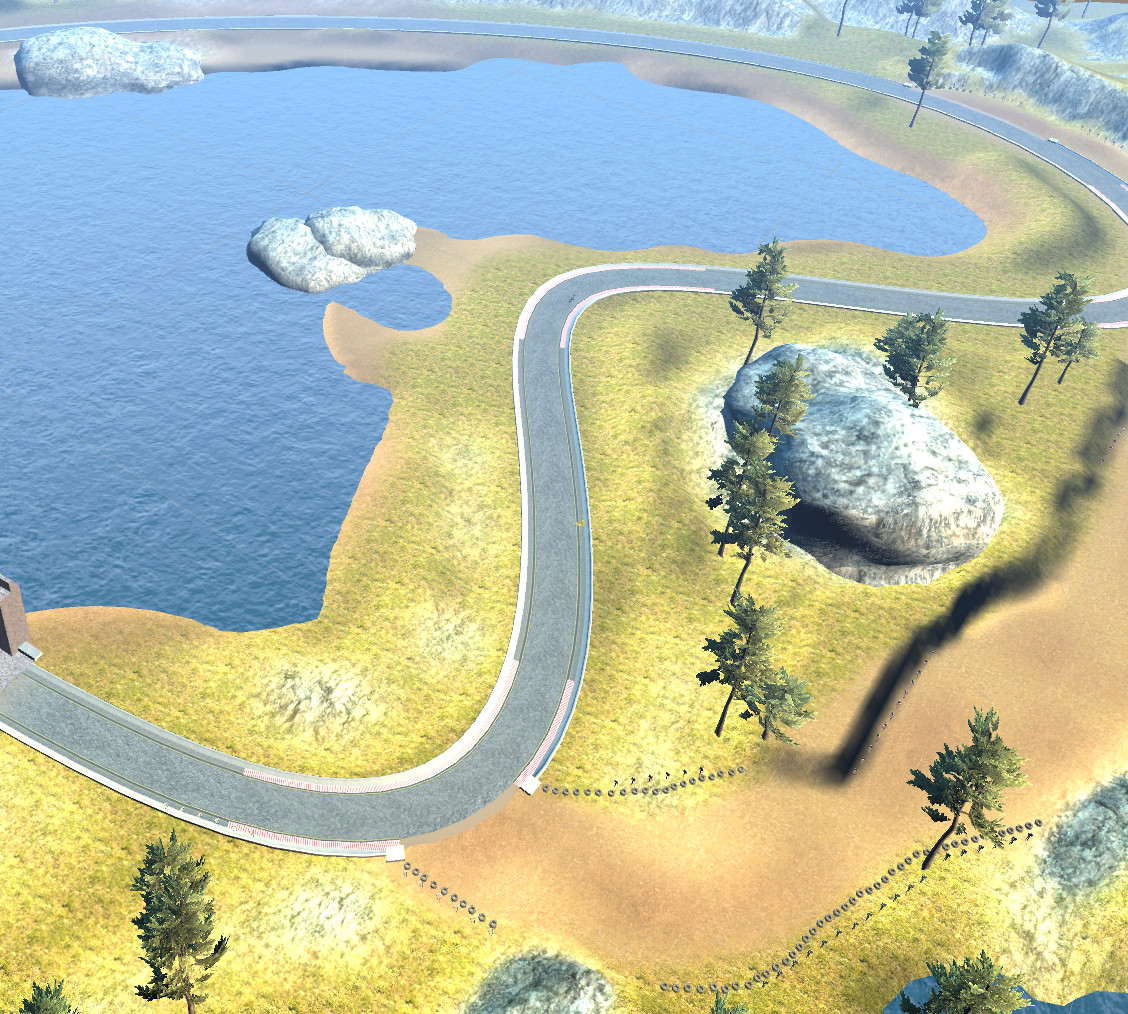
\includegraphics[height=5.5cm]{tracciato} }}%
    \caption{Le due ambientazioni del progetto}%
    \label{ambientazione}
\end{figure}
\vspace{-0.5cm}

\section{Unity}
\noindent 
\begin{wrapfigure}{r}{0.2\textwidth} %this figure will be at the right
    \centering
    \vspace{-1.3cm}
    
\includegraphics[height=3cm]{unityicon}
    \vspace{-1.3cm}
\end{wrapfigure}
Unity è un motore grafico integrato multipiattaforma per la creazione di videogiochi o altri contenuti interattivi 3D, quali visualizzazioni architettoniche o animazioni 3D in tempo reale. Unity permette di modellare l'ambientazione 3D e il modello della bicicletta virtuale attraverso script. Permette inoltre di integrare il visore per la Realtà Virtuale ed è per questo che la scelta è ricaduta su questo motore grafico: per via della facile integrazione dei visori quali OSVR e Oculus Rift.


\subsection{Schermata Principale}
\begin{figure}[htb]
    \centering
    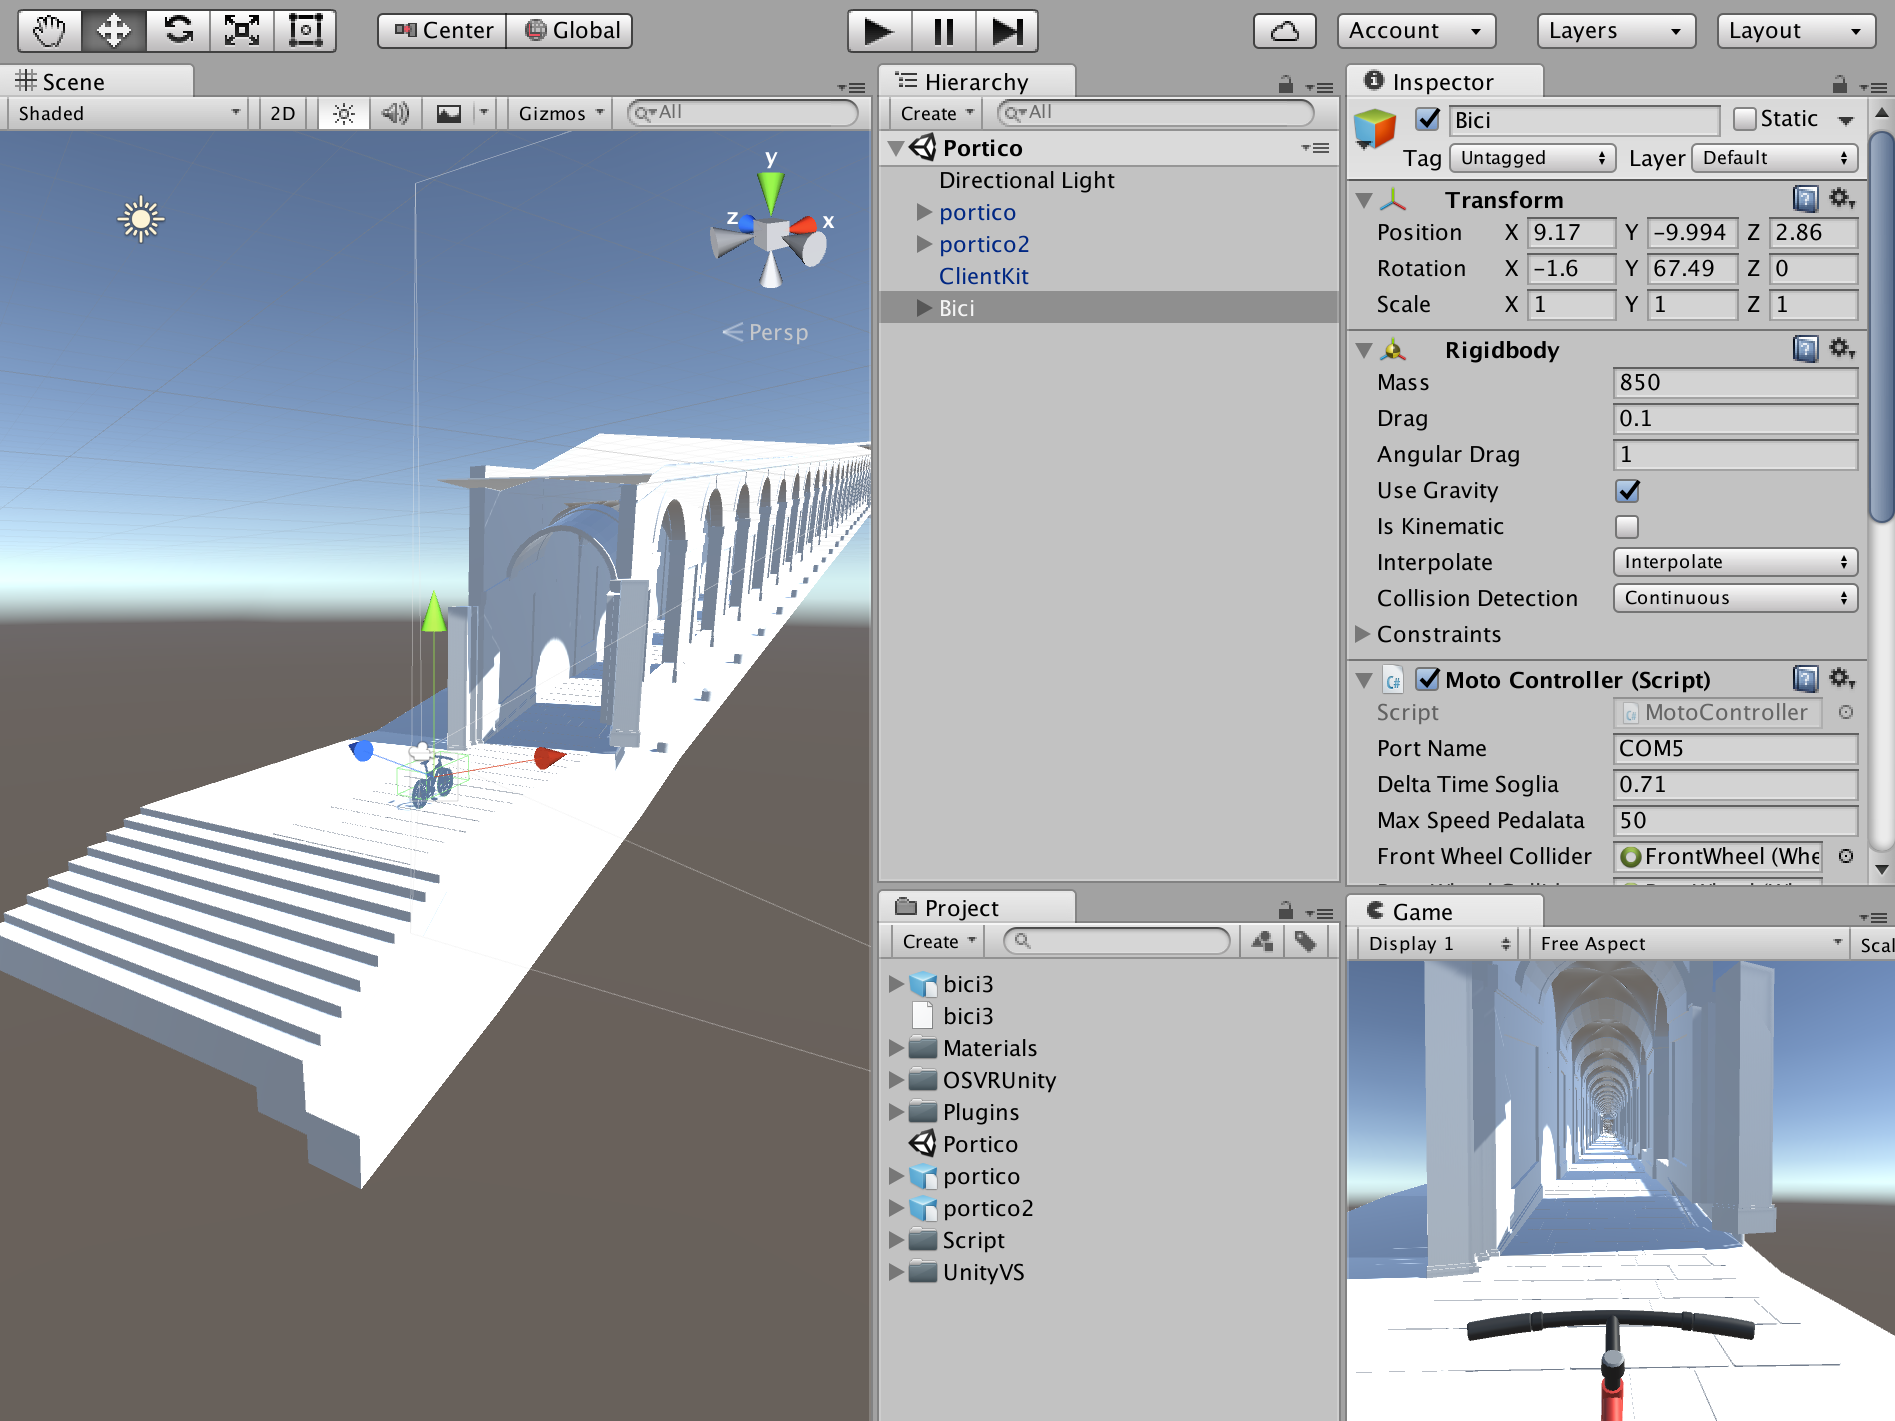
\includegraphics[width=\textwidth]{screenunity}
    \caption{La schermata principale di Unity\label{fig:screenunity}}
    \vspace{-0.3cm}
\end{figure}

\noindent La schermata principale di figura \nameref{fig:screenunity} si compone di 5 riquadri suddivisi in:
\begin{itemize}
  \item \textbf{Scene}: dove viene mostrata l'architettura dell'ambientazione e degli oggetti. All'interno di quest'area si ha la possibilità di modificare gli oggetti, scalarli, muoverli e/o ruotarli. È inoltre possibile cambiare visualizzazione e vista utilizzando mouse e tastiera.
 \item \textbf{Game}: in questo riquadro è possibile osservare l'inquadratura della telecamera o del visore quando la simulazione è avviata. È inoltre possibile interagire con tastiera per muovere gli oggetti o spostare la visuale.
  \item \textbf{Inspector}: questo pannello permette allo sviluppatore di modificare tutti i valori relativo ad un oggetto selezionato. Permette inoltre di assegnare script che modellino a tempo di esecuzione l'oggetto, come ad esempio modificandone la posizione e/o creando animazioni per muoverlo. 
  \item \textbf{Hierarchy}: in questo punto sono elencati tutti gli oggetti presenti nella scena in ordine di parentela o di directory. Ogni componente può averne al suo interno altre (figlie) e può essere usata per trasferire delle caratteristiche quali la posizione, la rotazione e/o vincolare quest'ultime ai comportamenti del padre. Grazie al pulsante Create si possono aggiungere nuovi elementi alla scena. Ogni elemento aggiunto può essere messo in gerarchia semplicemente trascinandolo su un altro con il mouse, questi possono essere oggetti 2D e 3D, telecamere, luci, ecc.
    \item \textbf{Project}: in questa sezione è possibile rintracciare tutte le cartelle e i file del progetto. Questa sezione può interagire con Hierarchy: è infatti possibile trascinare oggetti prefabbricati (come ad esempio la bicicletta creata in Blender) e posizionarli nella scena.
\end{itemize}
Ogni oggetto che fa parte del progetto è elencato all’interno del riquadro Project ed ogni oggetto che fa parte della scena si può trovare all’interno di Hierarchy. Gli oggetti all’interno di Hierarchy vengono chiamati GameObject e ognuno di questi può essere salvato come componente Prefab, con tutti i suoi figli, e riutilizzato in tutte le scene come oggetto identicamente uguale al GameObject che lo ha originato. Questa funzione risulta utile nel caso servano istanze multiple dello stesso GameObject all’interno di una o più scene. Quando viene modificato il GameObject originario, le variazioni si propagano a tutte le sue istanze nel programma. Selezionando un GameObject da Hierarchy o anche dalla sezione Project la finestra Inspector si adatta alla caratteristiche in esso contenute. Ogni GameObject possiede al suo interno dei Component che ne definiscono caratteristiche e comportamento.

\subsection{Scenario Principale}
Durante la progettazione sono stati eseguiti due distinti test su due scenari diversi. Il primo test è stato eseguito nel modello dei portici di San Luca ed è servito per testare il comportamento della bicicletta, in relazione alla fisica dell'attrito e dell'inerzia. Il motivo di questa scelta è dovuto alla pendenza dei portici, che portano la bicicletta a discendere per la gravità. Il secondo test è invece stato eseguito nel modello di un percorso di gara, per verificare l'efficenza della pedalata, la velocità e la pendenza della bicicletta durante una sterzata. Tutte le calibrazioni riguardanti la fisica si tratteranno nella sezione \textit{\nameref{sperimentazione}}. In questa sezione si descriverà lo scenario creato inizialmente per testare gli script che modellano il movimento della bicicletta a tempo di esecuzione.
 \begin{figure}[htb]
    \centering
    %\vspace{-0.7cm}
    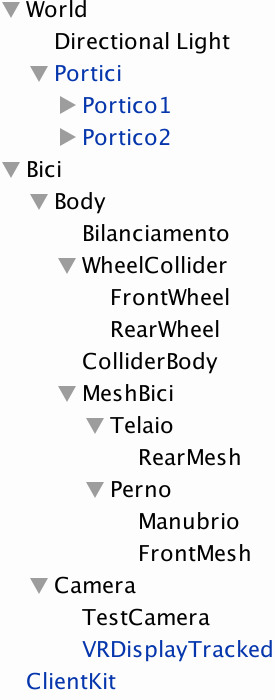
\includegraphics[height=8cm]{hierarchy}
    \caption{La gerarchia di GameObject nello scenario\label{fig:hierarchy}}
    %\vspace{-0.3cm}
\end{figure}
\noindent La gerarchia di GameObject nello scenario è la seguente.
\begin{itemize}
  \item \textbf{World}: Questo oggetto contiene tutti gli elementi del mondo virtuale. Contiene una luce direzionale e può contenere sia il modello dei portici, sia il modello del percorso di gara. Il modello dei portici di San Luca è stato fornito diviso in 2 parti, perciò questi sono stati riuniti in un unico oggetto padre che contiene i due sottogruppi di mesh. Il modello del percorso di gara è stato scaricato da internet come prefabbricato.
  \item \textbf{Bici}: l'oggetto padre contenente altri due oggetti:
		\begin{itemize}
  			\item \textbf{Body}: oggetto contenente le mesh e le meccaniche della bicicletta; i figli saranno vincolati a muoversi in concomitanza dei cambiamenti del suo Component Transform. Il body è un RigidBody: componente utilizzato per rappresentare la fisica dei GameObject composto da diversi dati. Tra i principali ritroviamo la massa assegnata, l’utilizzo o meno della gravità sul dato GameObject e le limitazioni di traslazione e rotazione. Al suo interno vi sono:
					\begin{itemize}
			  			\item \textit{Bilanciamento}: un oggetto che rappresenta il centro di massa della bicicletta su cui si concentrerà il peso. Questo è utile quando la bicicletta effettua salti, infatti le permette di non rovesciarsi.
			  			\item \textit{WheelCollider}: oggetto che contiene i collider delle due ruote, ovvero i GameObject che permettono di collidere con altri oggetti dello stesso tipo. Questi non permettono soloamente alla bicicletta di rimanere ancorata ad un terreno e di non attraversarlo, ma ruotando, forniscono anche il movimento.
						\item \textit{ColliderBody}: è stato aggiunto come involucro esterno per la collisione con l’ambiente circostante. Lo scopo è quello di rendere più realistico l'impatto, al momento della collisione della bici con i muri, evitando che le mesh visibili entrino per metà negli oggetti con cui si scontrano, prima di fermarsi.
						\item \textit{MeshBici}: contiene tutte le mesh della bicicletta. È suddiviso in due elementi: \textit{Telaio} e \textit{Perno}. Il telaio contiene la mesh della ruota posteriore e di tutto il telaio escluso il manubrio. Il perno è l'oggetto che contiene il manubrio e la mesh della ruota anteriore. È una mesh separata poiché permette in base a dove si deciderà di voltare, di avere un feedback visivo della scelta effettuata.
					\end{itemize}
			\item \textbf{Camera}: oggetto contenente due oggetti camera.   		\begin{itemize}
  						\item \textit{TestCamera}: camera solitamente disattivata. Utilizzata solamente in test senza il visore.
			  			\item \textit{VRDisplayTracked}: il Prefab\footnote{Oggetto prefabbricato di Unity, pronto per essere importato} del visore che sostituisce un normale oggetto camera. Questo oggetto camera permettere di essere ruotata tramite i movimenti del visore.
					\end{itemize}
		\end{itemize}
	\item \textbf{ClientKit}: Prefab di OSVR che si occupa del collegamento con il server e i relativi controlli tra il visore e il calcolatore.

\end{itemize}


\noindent Il funzionamento del WheelCollider è vincolato ad avere almeno un RigidBody come padre, questo sarà il componente sul quale verranno applicate tutte le forze di spostamento date dalla torsione delle ruote. Il RigidBody è stato impostato opportunamente ed è stato aggiunto uno script al GameObject per ricevere i segnali di input, per applicare forze alle ruote e per risolvere i limiti della fisica di Unity3D connessi ad esse. Lo script è stato generato vuoto aggiungendo il \textit{Component New Script} attraverso il tasto \textit{Add Component} nel riquadro \textit{Inspector}. Questo script è il \textit{MotoController} e fa uso di una classe \textit{DataReceiver} che si occupa di ricevere i dati dalla cyclette.

\newpage
\section{DataReceiver script}
Questa sezione descrive il comportamento dello script DataReceiver. Questo è stato fornito in versione completa nell'appendice \nameref{receiver} a pagina \pageref{receiver}. Lo script \textit{DataReceiver} si occupa di leggere i dati inviati dal microcontrollore della cyclette alla porta COM del computer e di interpretarli. È costituito da un costruttore, due funzioni private e due pubbliche:
\begin{itemize}
  \item \textbf{Costruttore}: permette di inizializzare la classe \textit{DataReceiver} per utilizzarla nella classe \textit{MotoController}. Esso inizializza il nome della porta COM utilizzata dal ricevitore Bluetooth e imposta la variabile pubblica \textit{go} a true. Questa variabile accessibile anche dal \textit{MotoController}, determina se il thread associato allo script deve continuare o no la lettura dalla porta.
\begin{lstlisting}{Costruttore}
public bool go;
private SerialPort serial;
private string _com;

public DataReceiver(string ComName) 
{
	go = true;
	_com = ComName;
}
\end{lstlisting}

  \item \textbf{Funzioni private}: queste funzioni si occupano di gestire la porta seriale COM.
\begin{itemize}
   \item \textbf{openPort}: si occupa di aprire la porta. Inizializza un oggetto \textit{SerialPort} a 9600bit/s di velocità, senza bit di parità, 8bit di dato e con un solo bit di stop. A questo oggetto assegna un buffer di lettura di dimensione 4096bit e abilita il Data Terminal Ready, un bit di controllo che può indicare l'intenzione di comunicare da parte del dispositivo. È stato necessario configurare un \textit{timeout} di 2 secondi alla lettura della porta. Questo per evitare che, alla chiusura dell'applicazione, il thread associato alla lettura rimanesse in attesa di un dato e bloccasse tutto il sistema. Infine viene fatta l'apertura della porta. La parte principale del metodo è riportata in seguito.
\begin{lstlisting}
serial = new SerialPort(_com, 9600, Parity.None, 8, StopBits.One);
serial.ReadBufferSize = 4096;
serial.DtrEnable = true;
serial.ReadTimeout = 2000; 		
serial.Open();
\end{lstlisting}

   \item \textbf{closePort}: si occupa della chiusura della porta seriale COM. Non fa altro che tentare di eseguire \texttt{serial.Close();} catturando eventuali eccezioni.
   \item \textbf{getData}: riceve e restituisce i dati della seriale sotto forma di stringa solo nel caso in cui lo script sia abilitato alla lettura, ovvero la variabile \textit{go} sia impostata a \textit{true}. Il codice eseguito è il seguente:
\begin{lstlisting}
String tmp = "";
if (serial.IsOpen && go)
	tmp = serial.ReadLine();
return tmp;
\end{lstlisting}
\end{itemize}%funzioni private

  \item \textbf{Funzioni pubbliche}: si basano sullo stato della variabile booleana \textit{go}. Se è \textit{true}, allora il processo abilitato alla lettura deve procedere, altrimenti deve chiudere la porta seriale e terminare la sua esecuzione. Queste funzioni sono richiamate ricorsivamente in \textit{MotoController} e utilizzano le funzioni private sopra definite.
\begin{itemize}
   \item \textbf{start}: apre la porta con \texttt{openPort} ed esegue \texttt{getData} iterativamente con un ciclo \textit{while}, finché \textit{go} è \textit{true}. Ogni volta che legge il dato, lo immagazzina in una stringa e lo suddivide in due valori: \textit{sterzo} e \textit{velocità} che poi invia ad Unity tramite l'evento \textit{PedalataTrovata}. Nel caso in cui \textit{go} sia \textit{false}, il processo esce dal ciclo ed esegue la chiusura della porta tramite \texttt{closePort}. La parsificazione eseguita all'interno del ciclo è descritta nel modo seguente(rimando alla sottosezione \textit{\nameref{stringa}} di pagina \pageref{stringa} per la composizione della stringa inviata dal microcontrollore):
\begin{lstlisting}
//gestione sterzo
tmp = "";
if (data[0] != '0')
tmp += data[0];
tmp += data[1];
sterzo = int.Parse(tmp);

//gestione velocita'
tmp = "";
if (data[3] != '0')
tmp += data[3];
tmp += data.Substring(4);
speed = float.Parse(tmp);
if (speed > 0 && data[2] == '-')
speed *= -1;

//Invio dati a unity
PedalataTrovata(sterzo, speed);
\end{lstlisting}

\item \textbf{stop}: semplicemente imposta la variabile \textit{go} a \textit{false}: \texttt{go = false;}. Questo obbliga il processo a terminare l'esecuzione uscendo dal ciclo \textit{while} sopra descritto.
\end{itemize}%funzioni pubbliche
\end{itemize}%funzioni
\newpage

\section{Motocontroller script}
Il \texttt{MotoController} è lo script direttamente applicato al GameObject \textit{Bici} e lo modella in relazione ai dati ricevuti dalla cyclette.
Al suo interno sono state inserite delle variabili pubbliche affinché siano accessibili direttamente dall’\textit{Inspector} in modo tale da poter aggiungere i vari GameObject di cui si necessita senza doverli cercare da codice. Unity3D al momento del lancio dell’applicazione si preoccupa di collegare alle variabili gli oggetti che sono stati registrati attraverso la schermata di progettazione, come si può vedere dall’immagine seguente.
 \begin{figure}[htb]
    \centering
    %\vspace{-0.7cm}
    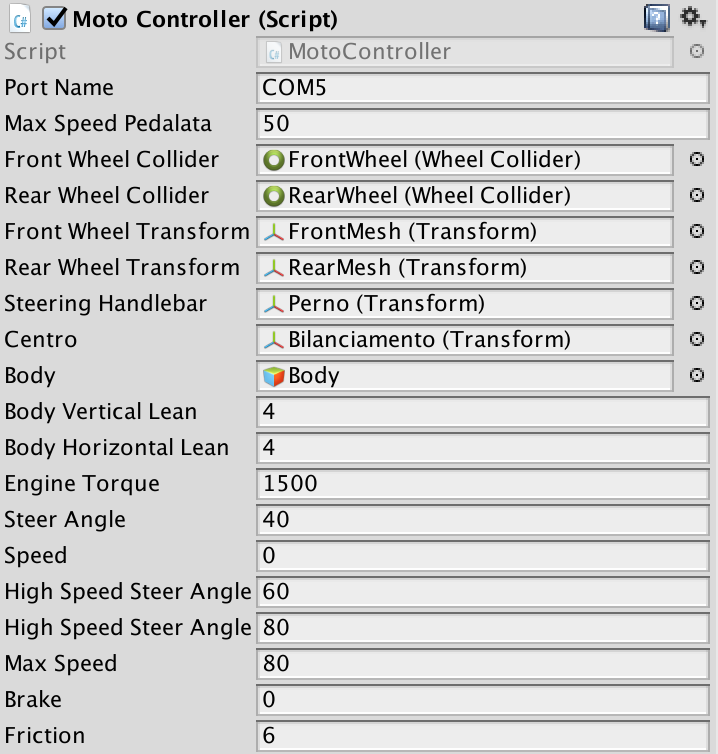
\includegraphics[height=8cm]{variabiliinspector}
    \caption{Le variabili impostabili direttamente dall'inspector di Unity\label{fig:variabiliinspector}}
    %\vspace{-0.3cm}
\end{figure}

\noindent Lo script è una classe che estende \texttt{MonoBehaviour}, una classe di default di Unity per modellare il comportamento di un GameObject. I campi dello Script MotoController.cs visibili nella schermata Inspector di Unity3D per il testing, sono:
\begin{itemize}
  \item Front/RearWheelCollider, rispettivamente i WheelCollider della ruota anteriore e posteriore.
  \item Front/RearWheelTransform, classi Transform collegate ai GameObject delle mesh delle ruote per i movimenti nello spazio e la rotazione della ruota anterore, in modo da dare l’effetto di movimento.
  \item SteeringHandleBar, Transform collegato alla mesh del manubrio per la rotazione nelle curve.
  \item Centro, componente per il calcolo del centro di massa.
  \item Body, GameObject che racchiude in sè tutti i componenti mobili appartenenti alla bici i quali dovranno inclinarsi durante una curva.
  \item Body Vertical Lean, vincolo sull’inclinazione verticale.
  \item Body Horizonatal Lean, vincolo per l’inclinazione orizzontale.
  \item Engine Torque, forza di torsione della ruota.
  \item Steer Angle, vincolo sull’angolo di sterzata massima.
  \item High Speed Steer Angle, angolo di sterzata ad alta velocità.
  \item High Speed Steer Angle At Speed, angolo di sterzata per velocità.
  \item Max Speed, limitatore di velocità.
  \item Brake, forza di frenata.
  \item Friction, forza di attrito.
\end{itemize}

\noindent Tutte le variabili giocano un ruolo fondamentale per il calcolo del movimento e la visualizzazione conseguente. All’interno delle funzioni che si mostreranno sotto, possiamo notarne il comportamento. Si è tuttavia omesso gran parte del codice per rendere più semplice la lettura di questa sezione. Si rimanda quindi all'appendice \nameref{controller} a pagina \pageref{controller}.
\begin{itemize}
	
	\item La funzione \texttt{Start} è la prima ad essere invocata subito dopo il popolamento delle variabili pubbliche, grazie ad essa è possibile:
  	\begin{itemize}
  		\item Salvare il collegamento al \textit{RigidBody}, in questo caso il GameObject, che contiene tutti gli altri, nella variabile \textit{rigid}.
  		\item Imporre vincoli sul movimento della rotazione dell’asse z, impedendo la rotazione.
  		\item Fissare il centro di massa calcolandolo partendo da quello standard e dal GameObject \textit{Bilanciamento}
  		\item Stabilire un limite alla velocità angolare
  		\item Salvare la preferenza per l’angolo di sterzata
  		\item Inizializzare il Receiver e impostare l'evento PedalataTrovata
  		\item Creare un thread separato che esegua il codice del Receiver.
	\end{itemize}
	
	\item \texttt{FixedUpdate} area che va utilizzata per la modifica dei GameObject che possiedono il Component RigidBody. All’interno invochiamo tre funzioni per il controllo degli input, quali l’attivazione del movimento delle ruote, l’eventuale arresto o retromarcia. Queste funzioni sono state definite sotto e sono:
		\begin{itemize}
			\item Inputs
			\item Engine
			\item Braking
		\end{itemize}
		
	\item \texttt{Update} viene richiamato in concomitanza con \texttt{Fixed\-Update} ed è indispensabile in quanto è l’unico metodo disponibile per l’aggiornamento dalla grafica. Al suo interno troviamo altre due funzioni utili per aggiornare i movimenti delle mesh su schermo e per controllare l’angolo del nostro assetto verticale:		\begin{itemize}
			\item WheelAlign
			\item Lean
		\end{itemize}
	
	\item \texttt{Inputs} controlla lo stato degli input e modifica le variabili che serviranno per calcolare il movimento che dovrà essere effettuato, nel dettaglio:
		\begin{itemize}
			\item Salva la velocità corrente convertita.
			\item Riporta i dati delle rotazioni imponendo quella sull’asse z a 0.
			\item Imposta la variabile che discrimina il movimento in avanti o all’indietro.
			\item Inserisce il valore della variabile per l’angolo di sterzata
			\item Controlla e imposta la variabile per la retromarcia.
		\end{itemize}
		
	\item \texttt{Engine} mette in moto i WheelCollider e permette quindi alla bicicletta di sostenere un moto accelerato. Il procedimento sarà quello di:
		\begin{itemize}
			\item Calcolare l’angolo di sterzata contenuta nelle variabili precedentemente ottenute grazie agli ingressi e imporle al Collider della ruota anteriore.
			\item Trovare la velocità da inserire. In base al valore che questa assume distinguiamo due comportamenti:
			\begin{itemize}
			  \item Il primo cessa l’accelerazione per il superamento della velocità massima, subendo l’inerzia fino al momento in cui non si torni al di sotto della soglia consentita riaccelerando.
			  \item Il secondo applica la forza di accelerazione il parametro \textit{motorTorque}
			\end{itemize}
			\item Controllare sul reversing: nel caso in cui l’input sia una velocità negativa, si impone questa pari a:
			\begin{itemize}
			  \item 0 per velocità maggiori di quella desiderata
			  \item una velocità di retromarcia ridotta.
			\end{itemize}
		\end{itemize}
		
		\item \texttt{Braking} in caso di frenata deceleriamo la bici fino al punto di invertire la marcia. Le opzioni sono:
		\begin{itemize}
			\item Se la velocità è inferiore da una certa soglia, rilasciando il tasto di input viene applicato un attrito che permetterà alla bici di fermarsi. Esso mantiene il mezzo fermo anche in caso di dislivello.
			\item Se applico un valore negativo di input e non siamo in retromarcia, si avrà una frenata più rapida.
			\item Se non si è in nessuno dei due precedenti casi, la forza di decelerazione viene resa nulla.
		\end{itemize}
		
		\item \texttt{WheelAlign} calcola i movimenti che dovranno eseguire le mesh delle ruote e del manubrio in accordo con l’input e i WheelCollider. Le fasi operative saranno:
		\begin{itemize}
			\item Calcolare il punto di contatto con il terreno.
			\item Controllare, tracciando una linea immaginaria dal centro della ruota, se lungo il percorso si incontra un altro Collider.
			\item Disegnare la mesh nel punto calcolato in base ai controlli effettuati.
			\item Adeguare la rotazione in base alla velocità e al tempo del movimento.
			\item Applicare la torsione alla ruota anteriore in base alla rotazione del FrontWheelCollider.
			\item Compiere i passaggi precedenti anche per la ruota posteriore, ovviamente trascurando la torsione derivante dal manubrio.
			\item Ruotare il manubrio in base all’angolo di sterzata. Siccome il manubrio è inclinato e non perfettamente perpendicolare al piano di appoggio, è stato necessario utilizzare Eulero attraverso i parametri \textit{eulerAngles}. Questo è quanto viene applicato:
			\begin{itemize}
			  \item Si ottiene la differenza di angolo tra la posizione corrente (euler.z) e l'angolo del FrontWheelCollider.
			  \item Si applica la formula \texttt{euler.z = \-(euler.z \-- \-angleDifference) \% 360} per fornire la rotazione sull'asse inclinato
			  \item Si applica il valore ottenuto agli \texttt{eulerAngles} del manubrio.
			\end{itemize}

		\end{itemize}
		
		\item \texttt{Lean} calcola e applica l’inclinazione verticale a fronte di una sterzata. Le operazioni contenute in essa sono:
		\begin{itemize}
			\item Calcolare l’angolo rispetto alla verticale in base ai dati e al tempo.
			\item Salvare i dati del contatto con il terreno del WheelCollider.
			\item Utilizzare i dati del contatto per ottenere l’angolo normalizzato in corrispondenza del terreno. Se quest’ultimo, dovesse essere maggiore, rispetto a quello desiderato, verrà limitato da un lato o dall’altro.
			\item Calcolare l’angolo orizzontale.
			\item Generare gli angoli di rotazione e applicarli al Body.
			\item Ricalcolare il centro di massa per non avere effetti anomali, per esempio di trascinamento orizzontale.
		\end{itemize}
		
		\item \texttt{ReceiverPedalataTrovata} funzione per gestire l'oggetto evento di \textit{DataReceiver} e aggiornare le variabili che immagazzinano i valori di sterzo e velocità di pedalata.
		\item \texttt{OnApplicationQuit} funzione che ridefinisce la chiusura dell'applicazione. Richiama la funzione \textit{stop} di \textit{DataReceiver} e si sospende in attesa della terminazione del thread associato.
		\item \texttt{msgToDebug} funzione utile per debug. Permette di scrivere direttamente nella console di debug, una stringa passata come argomento.
	
\end{itemize}

\noindent Un volta scritto, lo script \texttt{Motocontroller} deve essere associato all'oggetto Bici, come in figura \ref{fig:variabiliinspector}. 

\section{OSVR}
Il visore OSVR deve semplicemente sostituire l'oggetto camera con un suo prefabbricato. Questo prefabbricato è impostato per muoversi in relazione ai movimenti del visore. Per utilizzare i prefabbricati e per poter utilizzare il visore è stato necessario installare il software fornito dal portale sviluppatori su Github. I pacchetti che sono stati utilizzati sono tre: il primo per la configurazione del visore e per il controllo del suo funzionamento, il secondo per l'abilitazione dell'accelerometro e del giroscopio tramite l'utilizzo del server (un processo locale) e il terzo per importare sia i componenti da utilizzare sia le scene di testing all'interno di Unity. Utilizzando il secondo pacchetto contenente il server, un processo locale che utilizza un file .json per la configurazione del visore(e quindi è possibile crearsene di personalizzati), si è abilitato il tracker per il rilevamento della posizione e per lo spostamento dell'accelerometro. Completata la configurazione del visore, è stato possibile integrarlo con Unity. Dei componenti importati e necessari su Unity sono stati adoperati il \textit{ClientKit}, che si occupa del collegamento con il server e i relativi controlli tra il visore e il calcolatore, e il \textit{VRVRDisplayTracked} già dotato della camera, che consente di visualizzare la simulazione, e degli script per il movimento all'interno del mondo.


























%

\chapter{Sperimentazione e correzioni}
\label{sperimentazione}
\thispagestyle{empty}

%Si mostra il progetto dal punto di vista sperimentale, le cose materialmente realizzate. In questa sezione si mostrano le attivit\`a sperimentali svolte, si illustra il funzionamento del sistema (a grandi linee) e si spiegano i risultati ottenuti con la loro valutazione critica. Bisogna introdurre dati sulla complessit\`a degli algoritmi e valutare l'efficienza del sistema.

%discorso sulla fisica e di tutti i valori?

\section{Realizzazione del sistema}
Il sistema assemblato e impostato per il funzionamento si presenta come in figura.
 \begin{figure}[htb]
    \centering
    \vspace{-0.7cm}
    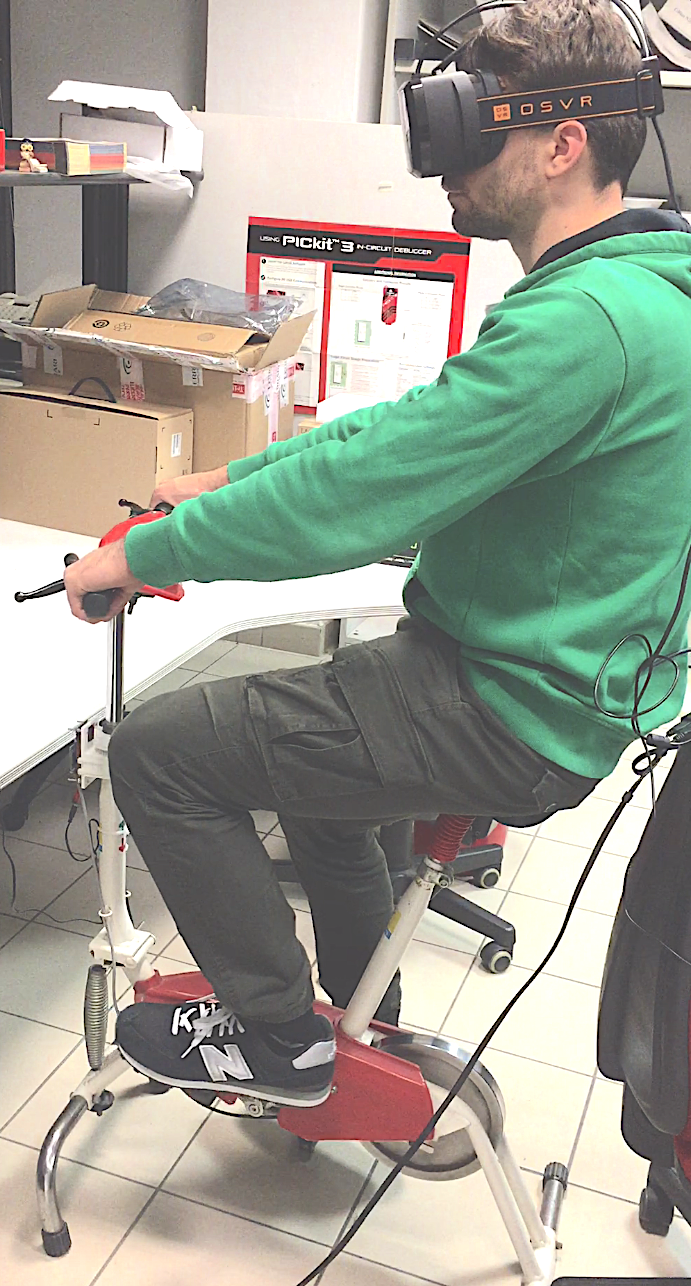
\includegraphics[height=11cm]{finale}
    \caption{Il sistema assemblato\label{fig:finale}}
    %\vspace{-0.3cm}
\end{figure}
\newpage
\noindent Per avere un corretto funzionamento di tutto il sistema è necessario seguire obbligatoriamente una determinata serie di operazioni nell'esatto ordine:
\begin{itemize}
  \item il computer principale deve essere accesso, deve avere il ricevitore bluetooth collegato e deve avere il progetto di Unity già pronto per essere avviato
  \item collegare alla corrente il microcontrollore della cyclette
  \item prendere l'hub dell'OSVR e collegarlo alla corrente
  \item collegare il visore all'hub
  \item prendere il cavo HDMI-USB dell'OSVR e collegare HDMI e USB all'hub
  \item prendere l'altra estremità del cavo e collegare l'usb al computer
  \item collegare l'HDMI al computer
  \item eseguire il server OSVR nel computer
  \item far partire l'applicazione premendo il tasto \textit{play} su Unity.
  \item Una volta partito, è necessario impostare a tutto schermo la schermata \textit{game}. Per farlo è necessario impostare nel modo corretto i monitor, poiché l'OSVR viene rilevato dal computer come un monitor secondario. È quindi necessario duplicare la stessa visione sui due monitor oppure spostare la schermata \textit{Game} nel monitor associato al visore.
  \item Può essere necessario utilizzare l'eseguibile ResetYaw (illustrato in seguito) per resettare l'orientazione del visore.
  \item A questo punto è possibile indossare il visore e cominciare ad utilizzare la bicicletta.
\end{itemize}

\newpage
\section{OSVR e le impostazioni iniziali}
\noindent Nei primi test eseguiti con l'OSVR appena installato, si è riscontrato un bug che, all'avviamento della simulazione, posizionava la telecamera ruotata di 90\degree verso destra e un inversione di rotazione tra roll (su Z) e pitch (su Y). La chiarificazione di questi movimenti si ha in figura \ref{fig:headmov}.
\begin{figure}[htb]
    \centering
    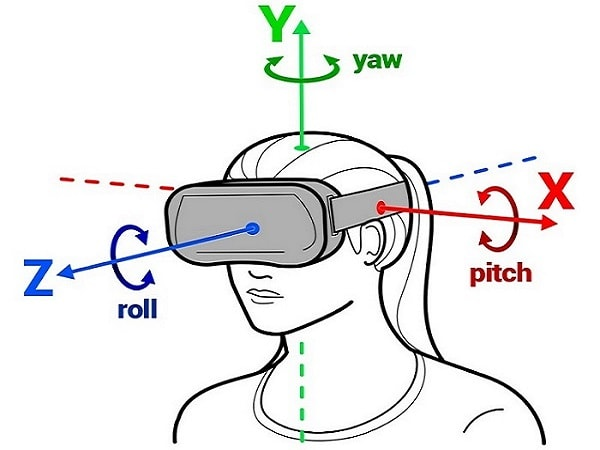
\includegraphics[height=8cm]{headmov}
    \caption{Le varie rotazioni della testa\label{fig:headmov}}
    \vspace{-0.3cm}
\end{figure}
\noindent Il problema è che l'OSVR necessita di una calibrazione iniziale che non era stata eseguita dopo l'installazione. Inizialmente si è risolto il problema posizionando la bicicletta a (0,0,0) con l'oggetto \textit{VRDisplayTracked} interno alla bicicletta con posizione (0,0,0) e tutte le rotazioni a 0. In questo modo le rotazioni a tempo di esecuzione erano tutte corrette. Tuttavia, esiste un tool fornito dal portale di sviluppo di OSVR che permette di resettare il sistema di coordinamento del visore, chiamato \textit{OSVRResetYaw}. Lanciando l'eseguibile di questo tool, è possibile resettare la posizione e le rotazioni del visore, portandolo ai valori impostati su Unity.

\section{Calibrazioni della fisica virtuale}
Testando la bicicletta nel tracciato di gara citato nella sottosezione \nameref{ambientazione} a pagina \pageref{ambientazione} si sono potuti definire al meglio i valori della fisica del mondo virtuale. I problemi principali erano: la velocità da fornire dopo una pedalata, l'inerzia e la frenata in caso di pedalata nulla. 
%Oltre a questi problemi principali è stata anche gestita la limitazione dello sterzo in caso di elevata velocità per evitare di perdere il controllo della bicicletta.

\subsection{Velocità}
La velocità è stata limitata al valore \textit{40} che rappresenta una velocità poco superiore alla realtà, ma rende realistico il modo in cui la bicicletta si muove nel mondo virtuale. Il valore \textit{MaxSpeedPedalata} è stato impostato a 20 e rappresenta, in modo inversamente proporzionale, quanto una pedalata può influire sulla velocità: più piccolo è, maggiore sarà l'accelerazione che ne deriva. Il valore che principalmente influenza la velocità della bicicletta è \textit{Engine Torque}. Questo è stato impostato a 1500 per avere una buona accelerazione ad ogni pedalata, ma è stato raggiunto per tentativi. Sotto i 1000 si otteneva una scarsa accelerazione, mentre sopra i 3000 si otteneva una velocità non realista che portava la bicicletta a inpennarsi. Per evitare l'effetto impennata è stato spostato l'oggetto \textit{Bilanciamento} fino ad un punto in cui la bicicletta non si ribaltava neanche durante dei salti.
 \begin{figure}[htb]
    \centering
    %\vspace{-0.7cm}
    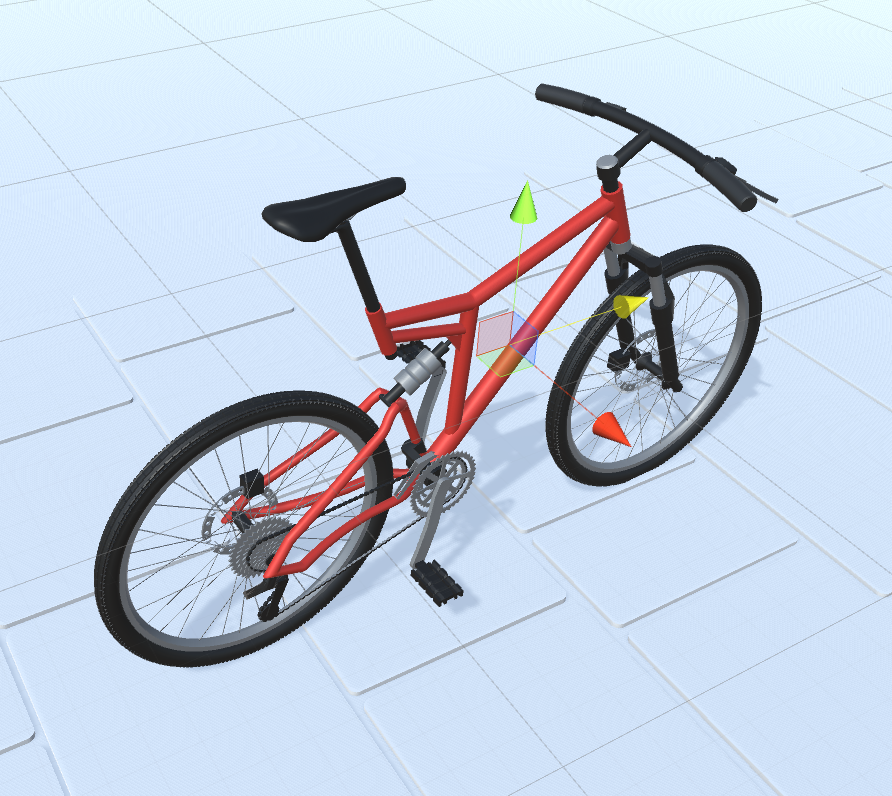
\includegraphics[height=8cm]{bilanciamento}
    \caption{Il punto in cui viene applicato il centro di massa\label{fig:bilanciamento}}
    %\vspace{-0.3cm}
\end{figure}

\subsection{Frenata e Inerzia}
I valori che influenzano la frenata sono \textit{Brake} e \textit{Friction}. Il primo è stato impostato a 2500 poiché con valori inferiori la bicicletta frena troppo lentamente e con valori superiori, faticava addirittura a partire. Il secondo è stato impostato a 6, poiché per valori molto superiori, la ruota posteriore slitta. Entrambi i valori sono stati impostati uno relativo all'altro durante la sperimentazione. L'inerzia viene gestita tramite questi valori nello script \texttt{MotoController} nella funzione \texttt{Braking}.

%\subsection{Sterzata}
%Per impedire che ad alte velocità






































%
\chapter{Direzioni future di ricerca e conclusioni}
\label{conclusioni}
\thispagestyle{empty}

%Si mostrano le prospettive future di ricerca nell'area dove si \`e svolto il lavoro. Talvolta questa sezione pu\`o essere l'ultima sottosezione della precedente. Nelle conclusioni si deve richiamare l'area, lo scopo della tesi, cosa \`e stato fatto,come si valuta quello che si \`e fatto e si enfatizzano le prospettive future per mostrare come andare avanti nell'area di studio.

\noindent 
L'obiettivo di questo progetto è creare un simulatore che permetta all'utente di pedalare ed immedesimarsi in un mondo virtuale. I risultati ottenuti nel tentativo di realizzare questo sistema sono discreti, ma non tanto realistici quanto voluto.
Per quanto possa essere accessibile, l'OSVR ha prestazioni piuttosto ridotte se viene utilizzato con ambientazioni con molti dettagli. Per la realtà virtuale è necessario un computer con elevate prestazioni e un visore con un'ottima risoluzione. Per la realizzazione del progetto non è stato possibile utilizzare strumenti con prestazioni migliori e senza questi, i risultati che si ottengono sono simulazioni non molto realistiche e spesso fastidiose. Infatti dopo diverse ore l'utente può accusare affaticamento alla vista, stanchezza e nello specifico cefalea e nausea.\\
Un altro problema è dovuto alla cyclette e al fatto che i dati ricavati dal suo utilizzo siano poco realistici. Non è infatti possibile fermare i piedi sui pedali affidandosi all'inerzia come in una reale bicicletta, poiché la cyclette ha i pedali direttamente ancorati al sistema del volano. Fermare i piedi sulla cyclette porta a fermare direttamente il volano, ma l'applicazione genera comunque l'inerzia sulla bicicletta virtuale. Inoltre, se nel modello vi fosse una salita, la bicicletta virtuale salirebbe più lentamente, ma l'utente che utilizza la cyclette non avrebbe nessun ritorno di forza dovuto alla pendenza.

\section{Soluzione}
Per sopperire a questi due problemi è in corso la progettazione di un sistema più sofisticato, che fa uso di una bicicletta vera e di rulli che permettano di dare un ritorno di forza in caso di pendenze. Un esempio è quello in figura.
 \begin{figure}[htb]
    \centering
    %\vspace{-0.7cm}
    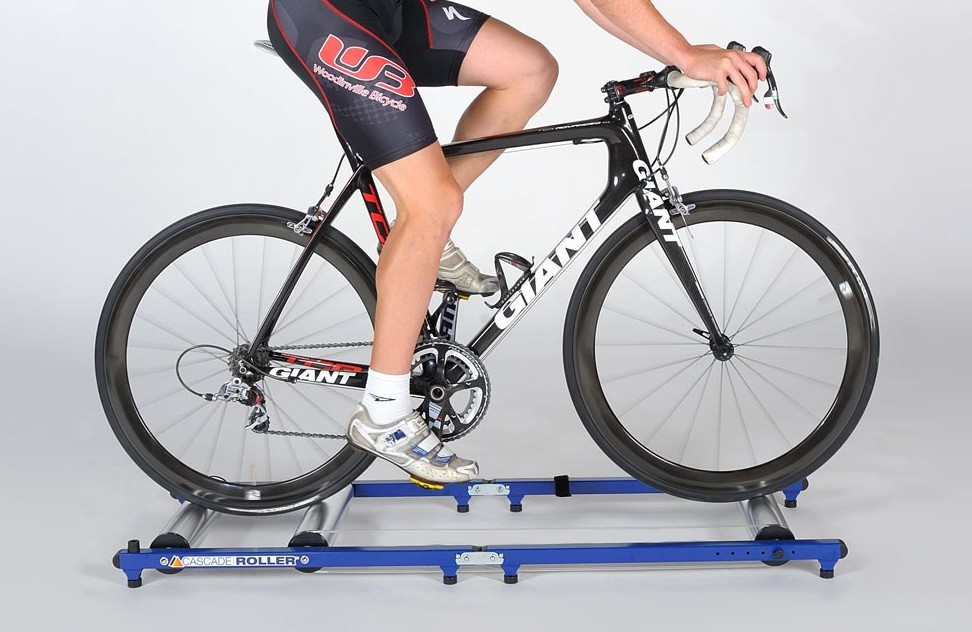
\includegraphics[height=8cm]{biciconrulli}
    \caption{Un esempio di bicicletta con rulli\label{fig:biciconrulli}}
    %\vspace{-0.3cm}
\end{figure}

\noindent Questi rulli avranno un modulo bluetooth che comunicherà con il calcolatore e riceverà da esso delle informazioni sulla pendenza del modello 3D. Inoltre, in futuro il sistema verrà aggiornato con visore molto più sofisticato: l'Oculus Rift. Questo visore ha una risoluzione più elevata e garantisce un'esperienza utente molto più realistica dell'OSVR. Tuttavia, necessita un computer con prestazioni molto più elevate. Verrà infatti installata, nel computer in laboratorio, una scheda video ASUS Strix NVidia GeForce GTX 1080, che è VR Ready, ovvero pronta per poter supportare la realtà virtuale e portare l'esperienza utente ai massimi livelli. Grazie alla popolarità di Unity, l'Oculus Rift è perfettamente integrabile ed esistono pacchetti che permettono di farlo con grande facilità.
\newpage
\section{Conclusioni}
Durante la progettazione, il lavoro è stato svolto con un occhio di riguardo alle future implementazioni. Si è quindi mantenuto un profilo generale anche nei dettagli, che permettesse una facile integrazione di una bicicletta vera. Nonostante la inevitabile eliminazione o variazione di tutto ciò che riguarda la cyclette e l'hardware associato, il simulatore software è già pronto per essere riutilizzato nel sistema con i rulli. L'unica modifica, di facile realizzazione, sarà quella di modificare la velocità in base alle informazioni che il sistema hardware fornirà riguardo alla pendenza. 
Gli sviluppi futuri e le integrazioni che si stanno applicando, porteranno il simulatore ad un livello di realismo considerevole, il quale potrà contribuire a portare la realtà virtuale nella vita di tutti i giorni.


\cleardoublepage

\appendix

\lstset{basicstyle=\ttfamily\scriptsize}

\chapter{Documentazione del progetto logico}
\label{appendiceA}
\thispagestyle{empty}

\noindent Documentazione del progetto logico dove si documenta il progetto logico del sistema e se \`e il caso si mostra la progettazione in grande del SW e dell'HW. Quest'appendice mostra l'architettura logica implementativa (nella Sezione 4 c'era la descrizione, qui ci vanno gli schemi a blocchi e i diagrammi).
\chapter{Codice script MotoController}
\label{controller}
\thispagestyle{empty}

\begin{lstlisting}
using UnityEngine;
using SerialLibrary;
using System.Threading;
using System.IO;

public class MotoController : MonoBehaviour {

    private SerialLibrary.DataReceiver receiver;
    private float pedalata;
    private float deltaTimePedalata;

    public string PortName = "COM5";
    
    public float deltaTimeSoglia = 0.71f;
    public float maxSpeedPedalata = 50.0f;

    private Rigidbody rigid;

    public WheelCollider FrontWheelCollider;
    public WheelCollider RearWheelCollider;
    public Transform FrontWheelTransform;
    public Transform RearWheelTransform;
	public Transform SteeringHandlebar;
    public Transform Centro;


    //Bike Body Lean
    public GameObject body;
    public float bodyVerticalLean = 10.0f;
    public float bodyHorizontalLean = 10.0f;
    private float horizontalLean = 0.0f;
    private float verticalLean = 0.0f;

    //Configurations
    public float EngineTorque = 1500f;

	[HideInInspector]
    public float SteerAngle = 30f;
    public float Speed;
    public float highSpeedSteerAngle = 40f;
    public float highSpeedSteerAngleAtSpeed = 80f;
    public float maxSpeed = 180f;
    public float Brake = 2500f;
    public float friction = 6f;

    private float motorInput = 0f;
    private float defsteerAngle = 0f;
    private float RotationValue1 = 0f;
    private float RotationValue2 = 0f;
	
	[HideInInspector]
    public float steerInput = 0f;
    private bool reversing = false;
    private float sterzata;
    private int lastInputSterzata;
    private float lastSterzata; 
    private Vector3 euler;
    private Vector3 FrontEuler;
    private Thread thread;

    void Start() {
        //Rigidbody
        rigid = GetComponent<Rigidbody>();
        rigid.constraints = RigidbodyConstraints.FreezeRotationZ;
        rigid.centerOfMass = new Vector3(Centro.localPosition.x * transform.localScale.x, Centro.localPosition.y * transform.localScale.y, Centro.localPosition.z * transform.localScale.z);
        rigid.maxAngularVelocity = 2f;
        
        defsteerAngle = SteerAngle;
        lastInputSterzata = 7;

        receiver = new DataReceiver(PortName);
        receiver.PedalataTrovata += Receiver_PedalataTrovata;
        thread = new Thread(receiver.start);

        euler = SteeringHandlebar.localEulerAngles;
        FrontEuler = FrontWheelTransform.localEulerAngles;

        thread.Start();
    }
 
    private void Receiver_PedalataTrovata(int inputSterzo, float inputPedalata)
    {
        if (lastInputSterzata == 0 && inputSterzo == 15)
            inputSterzo = 0;
            
        pedalata = inputPedalata/maxSpeedPedalata;

        sterzata = (inputSterzo - 7.0f) / 8; // Mathf.Lerp(lastSterzata, (inputSterzo - 7.0f) / 8, 0.2f);

        lastInputSterzata = inputSterzo;
        lastSterzata = sterzata;
    }

    void FixedUpdate()
    {
        Inputs();
        Engine();
        Braking();
    }

    void Update()
    {
        WheelAlign();
        Lean();
    }

    void Inputs()
    {
        Speed = rigid.velocity.magnitude * 3.6f;

        transform.eulerAngles = new Vector3(transform.eulerAngles.x, transform.eulerAngles.y, 0);

        motorInput = pedalata + Input.GetAxis("Vertical");
        steerInput = sterzata + Input.GetAxis("Horizontal");

        if (motorInput < 0)
            reversing = true;
        else
            reversing = false;

    }

    void Engine()
    {
        FrontWheelCollider.steerAngle = SteerAngle * steerInput;

        if (Speed > maxSpeed)
        {
            RearWheelCollider.motorTorque = 0;
        }
        else if (!reversing)
        {
            RearWheelCollider.motorTorque = EngineTorque * Mathf.Clamp(motorInput, 0f, 1f);
        }

        if (reversing)
        {
            if (Speed < maxSpeed)//test con 10
            {
                RearWheelCollider.motorTorque = (EngineTorque * motorInput) / 5f;
            }
            else
            {
                RearWheelCollider.motorTorque = 0;
            }
        }

    }

    public void Braking()
    {
        // Deceleration.
        if (Mathf.Abs(pedalata) <= .05f)
        {
            FrontWheelCollider.brakeTorque = (Brake) / friction; // 25f;
            RearWheelCollider.brakeTorque = (Brake) / friction; // 25f;
        }
        else if (motorInput < 0 && !reversing)
        {
            FrontWheelCollider.brakeTorque = (Brake) * (Mathf.Abs(motorInput) / 5f);
            RearWheelCollider.brakeTorque = (Brake) * (Mathf.Abs(motorInput));
        }
        else
        {
            FrontWheelCollider.brakeTorque = 0;
            RearWheelCollider.brakeTorque = 0;
        }

    }

    void WheelAlign()
    {
        RaycastHit hit;
        WheelHit CorrespondingGroundHit;
        float extension_F;
        float extension_R;

        Vector3 ColliderCenterPointFL = FrontWheelCollider.transform.TransformPoint(FrontWheelCollider.center);
        FrontWheelCollider.GetGroundHit(out CorrespondingGroundHit);

        if (Physics.Raycast(ColliderCenterPointFL, -FrontWheelCollider.transform.up, out hit, (FrontWheelCollider.suspensionDistance + FrontWheelCollider.radius) * transform.localScale.y))
        {
            if (hit.transform.gameObject.layer != LayerMask.NameToLayer("Bici"))
            {
                FrontWheelTransform.transform.position = hit.point + (FrontWheelCollider.transform.up * FrontWheelCollider.radius) * transform.localScale.y;
                extension_F = (
                -FrontWheelCollider.transform.InverseTransformPoint(
                CorrespondingGroundHit.point).y - FrontWheelCollider.radius) / FrontWheelCollider.suspensionDistance;
			}
        }
        else
        {
            FrontWheelTransform.transform.position = ColliderCenterPointFL - (FrontWheelCollider.transform.up * FrontWheelCollider.suspensionDistance) * transform.localScale.y;
        }
        //rotazione ruota anteriore: x fissa, y data dal movimento, z data dal perno
        RotationValue1 += FrontWheelCollider.rpm * (6) * Time.deltaTime;
        FrontEuler.x = 0;
        FrontEuler.y = -RotationValue1;
        FrontWheelTransform.localEulerAngles = FrontEuler;

        Vector3 ColliderCenterPointRL = RearWheelCollider.transform.TransformPoint(RearWheelCollider.center);
        RearWheelCollider.GetGroundHit(out CorrespondingGroundHit);

        if (Physics.Raycast(ColliderCenterPointRL, -RearWheelCollider.transform.up, out hit, (RearWheelCollider.suspensionDistance + RearWheelCollider.radius) * transform.localScale.y))
        {
            if (hit.transform.gameObject.layer != LayerMask.NameToLayer("Bici"))
            {
                RearWheelTransform.transform.position = hit.point + (RearWheelCollider.transform.up * RearWheelCollider.radius) * transform.localScale.y;
                extension_R = (
                -RearWheelCollider.transform.InverseTransformPoint(
                CorrespondingGroundHit.point).y - RearWheelCollider.radius) / RearWheelCollider.suspensionDistance;
			}
        } 
        else
        {
            RearWheelTransform.transform.position = ColliderCenterPointRL - (RearWheelCollider.transform.up * RearWheelCollider.suspensionDistance) * transform.localScale.y;
        }
        RotationValue2 += RearWheelCollider.rpm * (6) * Time.deltaTime;
        RearWheelTransform.transform.rotation = RearWheelCollider.transform.rotation * Quaternion.Euler(RotationValue2, RearWheelCollider.steerAngle, RearWheelCollider.transform.rotation.z+90);

        //rotazione del manubrio
		if (SteeringHandlebar) {
            //ottengo la differenza di angolo tra la posizione corrente (euler.z) e l'angolo della wheelcollider
            float angleDifference = euler.z - FrontWheelCollider.steerAngle;
            
            euler.z = (euler.z - angleDifference) % 360; //applico la differenza
            SteeringHandlebar.localEulerAngles = euler;  // aggiorno la rotazione
        }
    }

    void Lean()
    {
        verticalLean = Mathf.Clamp(Mathf.Lerp(verticalLean, transform.InverseTransformDirection(rigid.angularVelocity).x * bodyVerticalLean, Time.deltaTime * 5f), -10.0f, 10.0f);

        WheelHit CorrespondingGroundHit;
        FrontWheelCollider.GetGroundHit(out CorrespondingGroundHit);

        float normalizedLeanAngle = Mathf.Clamp(CorrespondingGroundHit.sidewaysSlip, -1f, 1f);

        if (transform.InverseTransformDirection(rigid.velocity).z > 0f)
            normalizedLeanAngle = -1;
        else
            normalizedLeanAngle = 1;

        horizontalLean = Mathf.Clamp(Mathf.Lerp(horizontalLean, (transform.InverseTransformDirection(rigid.angularVelocity).y * normalizedLeanAngle) * bodyHorizontalLean, Time.deltaTime * 3f), -50.0f, 50.0f);

        Quaternion target = Quaternion.Euler(verticalLean, body.transform.localRotation.y + (rigid.angularVelocity.z), horizontalLean);
        body.transform.localRotation = target;

        rigid.centerOfMass = new Vector3((Centro.localPosition.x) * transform.localScale.x, (Centro.localPosition.y) * transform.localScale.y, (Centro.localPosition.z) * transform.localScale.z);
    }

    void OnApplicationQuit()
    {
        receiver.stop();
        thread.Join();
        Debug.Log("Chiusura del programma: " + (thread.ThreadState));
    }

    public static void msgToDebug(string txt)
    {
        Debug.Log(txt);
 	}
}
\end{lstlisting}

%\cleartorightpage %commentare se vuoi margine esterno
\listoffigures

% ---- Bibliography ----
%\addcontentsline{toc}{chapter}{Bibliografia} //dà un errore
\bibliographystyle{plain}
\bibliography{bibl_tesi}
\nocite{*}


\end{document}





